% =====================================================================
%  Prof. Fang Math — Algebra 2, 6-7 Inverse Relations & Functions
%  One source file, two PDFs:
%    pdflatex -jobname=G7_Coordinate_Plane_Worksheet G7_Coordinate_Plane.tex
%    pdflatex -jobname=G7_Coordinate_Plane_Key "\def\iskey{1}% =====================================================================
%  Prof. Fang Math — Algebra 2, 6-7 Inverse Relations & Functions
%  One source file, two PDFs:
%    pdflatex -jobname=G7_Coordinate_Plane_Worksheet G7_Coordinate_Plane.tex
%    pdflatex -jobname=G7_Coordinate_Plane_Key "\def\iskey{1}% =====================================================================
%  Prof. Fang Math — Algebra 2, 6-7 Inverse Relations & Functions
%  One source file, two PDFs:
%    pdflatex -jobname=G7_Coordinate_Plane_Worksheet G7_Coordinate_Plane.tex
%    pdflatex -jobname=G7_Coordinate_Plane_Key "\def\iskey{1}% =====================================================================
%  Prof. Fang Math — Algebra 2, 6-7 Inverse Relations & Functions
%  One source file, two PDFs:
%    pdflatex -jobname=G7_Coordinate_Plane_Worksheet G7_Coordinate_Plane.tex
%    pdflatex -jobname=G7_Coordinate_Plane_Key "\def\iskey{1}\input{G7_Coordinate_Plane.tex}"
% =====================================================================
\documentclass[12pt,letterpaper]{article}
\usepackage[margin=0.8in,top=0.85in,bottom=0.8in]{geometry}
\usepackage{mathpazo}
\usepackage[T1]{fontenc}
\usepackage{amsmath,amssymb}
\usepackage{xcolor}
\usepackage{enumitem}
\usepackage{multicol}
\usepackage{booktabs}
\usepackage{needspace}
\usepackage{fancyhdr}
\usepackage[most]{tcolorbox}
\usepackage{pgfplots}
\pgfplotsset{compat=1.17}
\usetikzlibrary{arrows.meta,calc}

\definecolor{FangBlue}{HTML}{000000}
\definecolor{FangTeal}{HTML}{000000}
\definecolor{FangGold}{HTML}{555555}
\definecolor{FangRed}{HTML}{000000}
\definecolor{FangGreen}{HTML}{000000}
\definecolor{FangPurple}{HTML}{000000}
\definecolor{Soft}{HTML}{FFFFFF}

\newif\ifkey
\ifdefined\iskey \keytrue \else \keyfalse \fi

\pagestyle{fancy}\fancyhf{}
\renewcommand{\headrulewidth}{0.4pt}
\fancyhead[L]{\small\color{FangBlue}\textbf{Prof. Fang Math} \,|\, Grade 7 \,·\, Graphing on the Coordinate Plane}
\fancyhead[R]{\small\ifkey\textcolor{FangRed}{\textbf{ANSWER KEY}}\else Name: \underline{\hspace{4.2cm}}\fi}
\fancyfoot[C]{\small\thepage}
\fancyfoot[R]{\scriptsize\color{gray}fangmath.com}
\setlength{\headheight}{14pt}
\setlength{\parindent}{0pt}
\setlength{\parskip}{4pt}

% ---------- boxes ----------
\newtcolorbox{idea}[1][]{colback=Soft,colframe=FangBlue,boxrule=0.8pt,arc=3pt,left=8pt,right=8pt,top=6pt,bottom=6pt,
  fonttitle=\bfseries,coltitle=white,colbacktitle=FangBlue,title={#1}}
\newtcolorbox{example}[1][]{colback=white,colframe=FangTeal,boxrule=0.6pt,arc=3pt,left=8pt,right=8pt,top=5pt,bottom=5pt,
  fonttitle=\bfseries,coltitle=FangTeal,colbacktitle=white,title={#1},attach boxed title to top left={xshift=8pt,yshift=-7pt},boxed title style={boxrule=0pt,colframe=white}, enhanced}
\newtcolorbox{warn}{colback=FangRed!5,colframe=FangRed,boxrule=0.6pt,arc=3pt,left=8pt,right=8pt,top=4pt,bottom=4pt,leftrule=3pt}
\newtcolorbox{simple}{colback=FangGold!10,colframe=FangGold,boxrule=0.6pt,arc=3pt,left=8pt,right=8pt,top=4pt,bottom=4pt,leftrule=3pt}
\newtcolorbox{sol}{colback=FangGreen!6,colframe=FangGreen,boxrule=0.5pt,arc=2pt,left=6pt,right=6pt,top=3pt,bottom=3pt,breakable}

\newcommand{\badge}[2]{\tcbox[on line,colback=#1,colframe=#1,coltext=white,boxrule=0pt,arc=6pt,left=4pt,right=4pt,top=1pt,bottom=1pt,fontupper=\scriptsize\bfseries]{#2}}
\newcommand{\easy}{\badge{FangGreen}{EASY}}
\newcommand{\medium}{\badge{FangTeal}{MEDIUM}}
\newcommand{\hard}{\badge{FangRed}{HARD}}
\newcommand{\work}[2][]{\ifkey\begin{sol}#2\end{sol}\else\vspace*{#1}\fi}
\newcommand{\np}[1][6cm]{\needspace{#1}}
\newcommand{\sect}[2]{\par\needspace{7cm}\medskip{\Large\bfseries\color{FangBlue}\tcbox[on line,colback=FangBlue,colframe=FangBlue,coltext=white,arc=2pt,boxrule=0pt,left=5pt,right=5pt,top=1pt,bottom=1pt]{#1}\ #2}\par\smallskip}

% ---------- right-triangle picture: \rt{scale}{a}{b}{labels...} ----------
% vertices: C = right angle at origin, A = (b,0) [the angle we look from], B = (0,a)
% ---------- coordinate grid: \cg[size]{xmin}{xmax}{ymin}{ymax}{plot commands} ----------
\newcommand{\cg}[6][5.4cm]{\begin{tikzpicture}\begin{axis}[width=#1,height=#1,axis lines=middle,
  xmin=#2-0.6,xmax=#3+0.6,ymin=#4-0.6,ymax=#5+0.6,xtick={#2,...,#3},ytick={#4,...,#5},
  grid=both,grid style={gray!28},xlabel={\scriptsize$x$},ylabel={\scriptsize$y$},
  tick label style={font=\tiny},axis line style={-{Stealth[length=4pt]},thick},clip=false,
  xticklabel style={fill=white,inner sep=1pt},yticklabel style={fill=white,inner sep=1pt}]#6\end{axis}\end{tikzpicture}}
\newcommand{\pt}[4][FangBlue]{\fill[#1](axis cs:#2,#3) circle(2.3pt) node[above right,font=\scriptsize\bfseries,text=#1,inner sep=1.5pt]{#4};}
\newcommand{\blank}{\underline{\hspace{1.6cm}}}

\begin{document}

% ======================= TITLE =======================
\begin{center}
{\color{FangBlue}\Huge\bfseries Graphing on the Coordinate Plane}\\[3pt]
{\large Test review: points, quadrants, reflections, distance, shapes and proportional graphs}
\ifkey\\[3pt]{\color{FangRed}\large\bfseries Answer Key}\fi
\end{center}
\vspace{-2pt}

% ======================= PART 1 =======================
\sect{1}{The coordinate plane}

\begin{minipage}[c]{0.46\textwidth}\centering
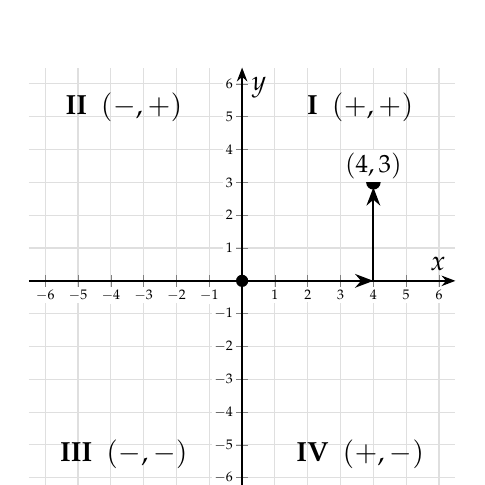
\begin{tikzpicture}
\begin{axis}[width=7cm,height=7cm,axis lines=middle,xmin=-6.5,xmax=6.5,ymin=-6.5,ymax=6.5,
  xtick={-6,...,6},ytick={-6,...,6},grid=both,grid style={gray!25},xlabel={$x$},ylabel={$y$},
  tick label style={font=\tiny},axis line style={-{Stealth[length=5pt]},thick},
  xticklabel style={fill=white,inner sep=1pt},yticklabel style={fill=white,inner sep=1pt}]
\node[FangTeal,font=\bfseries] at (axis cs:3.6,5.3) {I \ $(+,+)$};
\node[FangTeal,font=\bfseries] at (axis cs:-3.6,5.3) {II \ $(-,+)$};
\node[FangTeal,font=\bfseries] at (axis cs:-3.6,-5.3) {III \ $(-,-)$};
\node[FangTeal,font=\bfseries] at (axis cs:3.6,-5.3) {IV \ $(+,-)$};
\draw[FangRed,thick,-{Stealth}] (axis cs:0,0) -- (axis cs:4,0);
\draw[FangRed,thick,-{Stealth}] (axis cs:4,0) -- (axis cs:4,2.85);
\fill[FangRed](axis cs:4,3) circle(2.6pt) node[above,font=\small\bfseries,fill=white,inner sep=1pt]{$(4,3)$};
\fill(axis cs:0,0) circle(2.2pt);
\end{axis}
\end{tikzpicture}
\end{minipage}\hfill
\begin{minipage}[c]{0.52\textwidth}
\begin{itemize}[leftmargin=*,itemsep=3pt]
\item The \textbf{$x$-axis} goes left–right; the \textbf{$y$-axis} goes up–down. They cross at the \textbf{origin} $(0,0)$.
\item An \textbf{ordered pair} $(x,\,y)$: \textbf{first} walk left/right ($x$), \textbf{then} up/down ($y$). \\
\emph{“Walk to the elevator, then ride it.”}
\item The axes cut the plane into four \textbf{quadrants}, numbered I–IV \textbf{counterclockwise}, starting at the top right.
\item A point \textbf{on an axis} (like $(0,5)$ or $(-2,0)$) is in \textbf{no} quadrant.
\end{itemize}
\end{minipage}

\begin{warn}
\textbf{Watch out:} $(4,3)$ and $(3,4)$ are \textbf{different} points. Order matters: $x$ always comes first.
\end{warn}

% ======================= PART 2 =======================
\sect{2}{Reflections — flip over an axis}

\begin{minipage}[c]{0.46\textwidth}\centering
\cg[6.4cm]{-5}{5}{-5}{5}{
\pt[FangBlue]{3}{2}{$A(3,2)$}
\fill[FangRed](axis cs:3,-2) circle(2.3pt) node[below right,font=\scriptsize\bfseries,text=FangRed]{$(3,-2)$};
\fill[FangGreen](axis cs:-3,2) circle(2.3pt) node[above left,font=\scriptsize\bfseries,text=FangGreen]{$(-3,2)$};
\draw[FangRed,dashed](axis cs:3,2)--(axis cs:3,-2);
\draw[FangGreen,dashed](axis cs:3,2)--(axis cs:-3,2);}
\end{minipage}\hfill
\begin{minipage}[c]{0.52\textwidth}
\renewcommand{\arraystretch}{1.35}
\begin{tabular}{@{}lll@{}}
\toprule
\textbf{Reflect over\ldots} & \textbf{Rule} & \textbf{Example}\\ \midrule
\textcolor{FangRed}{the $x$-axis} & $(x,y)\to(x,\,-y)$ & $(3,2)\to(3,-2)$\\
\textcolor{FangGreen}{the $y$-axis} & $(x,y)\to(-x,\,y)$ & $(3,2)\to(-3,2)$\\
\bottomrule
\end{tabular}\par\medskip
\textbf{Memory trick:} over the \textbf{$x$-axis}, the \textbf{$x$ stays}; only $y$ changes sign. Over the \textbf{$y$-axis}, the \textbf{$y$ stays}.
\end{minipage}

% ======================= PART 3 =======================
\sect{3}{Distance between two points on a line}

\begin{idea}[Same $x$ or same $y$? Count — or use absolute value]
\textbf{Same quadrant / same side:} subtract. \quad $(2,5)$ to $(2,1)$: \ $5-1=4$ units.\par
\textbf{Opposite sides of an axis:} \textbf{add} the absolute values. \quad $(-3,4)$ to $(5,4)$: \ $|-3|+|5|=3+5=8$ units.\par
One rule for both: \textbf{distance} $=|\,\text{difference}\,|$. \quad $|5-(-3)|=|8|=8$. \ \ Distance is never negative.
\end{idea}

\begin{simple}
\textbf{Simple case first:} from $(-1,0)$ to $(1,0)$ — count the squares: $2$. And $|-1|+|1|=2$ \checkmark. That's why you \textbf{add} across the axis.
\end{simple}

% ======================= PART 4 =======================
\sect{4}{Shapes on the coordinate plane}

\begin{example}[Example \;·\; rectangle $ABCD$ with $A(-3,2)$, $B(4,2)$, $C(4,-1)$, $D(-3,-1)$]
\begin{minipage}[c]{0.4\textwidth}\centering
\cg[5.6cm]{-4}{5}{-2}{3}{
\draw[FangBlue,thick,fill=FangBlue!8](axis cs:-3,2)--(axis cs:4,2)--(axis cs:4,-1)--(axis cs:-3,-1)--cycle;
\pt{-3}{2}{A}\pt{4}{2}{B}\pt{4}{-1}{C}\pt{-3}{-1}{D}}
\end{minipage}\hfill
\begin{minipage}[c]{0.56\textwidth}
Length $AB$: same $y$, so $|4-(-3)|=7$. \\
Width $BC$: same $x$, so $|2-(-1)|=3$. \\[3pt]
\textbf{Perimeter} $=7+3+7+3=20$ units. \\
\textbf{Area} $=7\times3=21$ square units.
\end{minipage}
\end{example}

% ======================= PART 5 =======================
\sect{5}{Graphing a proportional relationship}

\begin{example}[Example \;·\; Tickets cost \$3 each]
\begin{minipage}[c]{0.42\textwidth}\centering
\begin{tabular}{c|ccccc}
tickets $x$ & 0 & 1 & 2 & 3 & 4\\ \hline
cost $y$ (\$) & 0 & 3 & 6 & 9 & 12
\end{tabular}\\[6pt]
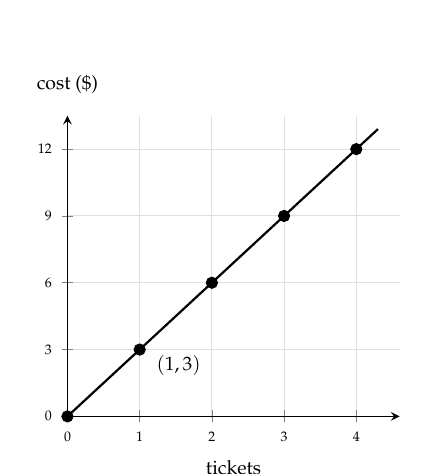
\begin{tikzpicture}
\begin{axis}[width=5.8cm,height=5.4cm,axis lines=left,xmin=0,xmax=4.6,ymin=0,ymax=13.5,xtick={0,...,4},ytick={0,3,...,12},
  grid=both,grid style={gray!25},xlabel={\scriptsize tickets},ylabel={\scriptsize cost (\$)},tick label style={font=\tiny},
  ylabel style={rotate=-90,at={(axis description cs:0,1.04)},anchor=south}]
\addplot[FangBlue,thick,domain=0:4.3]{3*x};
\addplot[only marks,mark=*,mark options={fill=FangBlue,draw=FangBlue}] coordinates{(0,0)(1,3)(2,6)(3,9)(4,12)};
\node[FangRed,font=\scriptsize\bfseries,anchor=west] at (axis cs:1.1,2.3) {$(1,3)$};
\end{axis}
\end{tikzpicture}
\end{minipage}\hfill
\begin{minipage}[c]{0.55\textwidth}
\textbf{How to tell it's proportional from a graph:}
\begin{enumerate}[leftmargin=*,itemsep=2pt]
\item the points are on a \textbf{straight line}, and
\item the line goes \textbf{through the origin} $(0,0)$.
\end{enumerate}
The \textbf{constant of proportionality} (unit rate) is $k=\dfrac{y}{x}=\dfrac{3}{1}=3$. Equation: $y=3x$.\par
\textbf{Look for the point $(1,\,k)$}: here $(1,3)$ means \emph{1 ticket costs \$3}.\par
A point like $(4,12)$ means \emph{4 tickets cost \$12}.
\end{minipage}
\end{example}

\begin{warn}
\textbf{Not proportional:} a straight line that \textbf{doesn't} pass through $(0,0)$ — for example a \$5 entry fee plus \$3 per ride: $y=3x+5$ starts at $(0,5)$.
\end{warn}

% ======================= PRACTICE =======================
\sect{6}{Practice}
\ifkey\else\textit{Show your work. Label every point you plot.}\fi

\needspace{8cm}{\large\bfseries\color{FangBlue}A.\ Read and plot points} \easy

\begin{minipage}[t]{0.42\textwidth}\vspace{0pt}\centering
\cg[6.2cm]{-6}{6}{-6}{6}{
\pt{2}{5}{A}\pt{-4}{3}{B}\pt{-3}{-2}{C}\pt{5}{-4}{D}\pt{0}{-5}{E}\pt{-6}{0}{F}
\ifkey
\pt[FangRed]{3}{1}{P}\pt[FangRed]{-5}{-4}{Q}\pt[FangRed]{0}{4}{R}\pt[FangRed]{4}{-2}{S}
\fi}
\end{minipage}\hfill
\begin{minipage}[t]{0.55\textwidth}\vspace{2pt}
\begin{enumerate}[leftmargin=*,label=\textbf{\arabic*.},itemsep=5pt]
\item Write the coordinates of each point.\\[3pt]
$A$ \ifkey\textcolor{FangGreen}{$(2,5)$}\else\blank\fi \quad $B$ \ifkey\textcolor{FangGreen}{$(-4,3)$}\else\blank\fi \\[3pt]
$C$ \ifkey\textcolor{FangGreen}{$(-3,-2)$}\else\blank\fi \quad $D$ \ifkey\textcolor{FangGreen}{$(5,-4)$}\else\blank\fi \\[3pt]
$E$ \ifkey\textcolor{FangGreen}{$(0,-5)$}\else\blank\fi \quad $F$ \ifkey\textcolor{FangGreen}{$(-6,0)$}\else\blank\fi
\item Which quadrant is each of $A$, $B$, $C$, $D$ in? Which points are on an axis?
\work[1.2cm]{$A$: I, \ $B$: II, \ $C$: III, \ $D$: IV. \ $E$ and $F$ are on an axis (no quadrant).}
\item Plot and label on the same grid: \\ $P(3,1)$, \ $Q(-5,-4)$, \ $R(0,4)$, \ $S(4,-2)$.
\work[0.4cm]{Points $P$, $Q$, $R$, $S$ are plotted on the grid.}
\end{enumerate}
\end{minipage}

\needspace{5cm}{\large\bfseries\color{FangBlue}B.\ Signs and quadrants} \easy\ \medium

\begin{enumerate}[start=4,leftmargin=*,label=\textbf{\arabic*.},itemsep=5pt]
\np[2cm]\item Name the quadrant: \quad (a) $(-7,\,2)$ \quad (b) $(6,\,-1)$ \quad (c) $(-0.5,\,-8)$ \quad (d) $(3\tfrac12,\,4)$
\work[1cm]{(a) II \quad (b) IV \quad (c) III \quad (d) I}
\np[2cm]\item A point has a negative $x$-coordinate and a positive $y$-coordinate. Which quadrant is it in?
\work[1cm]{Quadrant II \ $(-,+)$.}
\np[2cm]\item True or false: the point $(0,-3)$ is in Quadrant IV. Explain.
\work[1.2cm]{False. Its $x$-coordinate is $0$, so it lies \textbf{on the $y$-axis} — in no quadrant.}
\end{enumerate}

\needspace{5cm}{\large\bfseries\color{FangBlue}C.\ Reflections} \medium

\begin{enumerate}[resume,leftmargin=*,label=\textbf{\arabic*.},itemsep=5pt]
\np[2cm]\item Reflect $(5,-2)$ over the $x$-axis. \quad Then reflect $(5,-2)$ over the $y$-axis.
\work[1cm]{Over the $x$-axis: $(5,2)$. \quad Over the $y$-axis: $(-5,-2)$.}
\np[2cm]\item $(-4,\,6)$ is reflected over the $y$-axis, and then the new point is reflected over the $x$-axis. Where does it end up? Which quadrant?
\work[1.4cm]{$(-4,6)\to(4,6)\to(4,-6)$. \ Quadrant IV. (Two flips change both signs.)}
\np[2cm]\item Point $M$ is $(a,\,b)$ and point $N$ is $(a,\,-b)$. Over which axis is $N$ the reflection of $M$?
\work[1cm]{The $x$-axis (the $x$-coordinate stayed the same).}
\end{enumerate}

\needspace{5cm}{\large\bfseries\color{FangBlue}D.\ Distance} \medium

\begin{enumerate}[resume,leftmargin=*,label=\textbf{\arabic*.},itemsep=5pt]
\np[2cm]\item Find the distance between $(3,\,7)$ and $(3,\,-2)$.
\work[1.2cm]{Same $x$. Opposite sides of the $x$-axis: $7+2=9$ units. \ (Or $|7-(-2)|=9$.)}
\np[2cm]\item Find the distance between $(-6,\,-1)$ and $(-2,\,-1)$.
\work[1.2cm]{Same $y$. Same side: $|-2-(-6)|=|4|=4$ units.}
\np[2cm]\item Point $A$ is at $(-5,\,4)$. Point $B$ is $9$ units to the right of $A$. Find $B$. Which quadrant is $B$ in?
\work[1.2cm]{$B=(-5+9,\,4)=(4,4)$, \ Quadrant I.}
\np[2.4cm]\item A diver is at $-12$ m and a seagull is at $+15$ m, straight above the diver. How far apart are they?
\work[1.2cm]{$|-12|+|15|=12+15=27$ m (opposite sides of sea level, so add).}
\end{enumerate}

\needspace{7cm}{\large\bfseries\color{FangBlue}E.\ Shapes} \medium\ \hard

\begin{enumerate}[resume,leftmargin=*,label=\textbf{\arabic*.},itemsep=6pt]
\np[5cm]\item \begin{minipage}[t]{0.5\textwidth}\vspace{0pt}
Plot $J(-4,3)$, $K(2,3)$, $L(2,-2)$ and $M(-4,-2)$ and connect them in order. \\
(a) What shape is $JKLM$? \\ (b) Find its perimeter. \\ (c) Find its area.
\work[0.2cm]{(a) A rectangle. \ (b) $JK=|2-(-4)|=6$, $KL=|3-(-2)|=5$. Perimeter $=2(6+5)=22$ units. \ (c) Area $=6\times5=30$ square units.}
\end{minipage}\hfill
\begin{minipage}[t]{0.42\textwidth}\vspace{0pt}\centering
\cg[5.6cm]{-5}{5}{-5}{5}{\ifkey\draw[FangBlue,thick,fill=FangBlue!8](axis cs:-4,3)--(axis cs:2,3)--(axis cs:2,-2)--(axis cs:-4,-2)--cycle;\pt{-4}{3}{J}\pt{2}{3}{K}\pt{2}{-2}{L}\pt{-4}{-2}{M}\fi}
\end{minipage}
\np[2.6cm]\item Three corners of a square are $(-1,4)$, $(3,4)$ and $(3,0)$. Find the fourth corner and the area of the square.
\work[1.4cm]{The fourth corner is $(-1,0)$. Side $=|3-(-1)|=4$, so area $=4\times4=16$ square units.}
\np[3cm]\item \hard\ A triangle has vertices $(-2,-3)$, $(4,-3)$ and $(1,5)$. Find its area.
\work[1.6cm]{Base on $y=-3$: $|4-(-2)|=6$. Height: from $y=-3$ up to $y=5$ is $|5-(-3)|=8$. \ Area $=\tfrac12\cdot6\cdot8=24$ square units.}
\end{enumerate}

\needspace{8cm}{\large\bfseries\color{FangBlue}F.\ Proportional relationships} \medium\ \hard

\begin{enumerate}[resume,leftmargin=*,label=\textbf{\arabic*.},itemsep=6pt]
\np[6.5cm]\item \begin{minipage}[t]{0.52\textwidth}\vspace{0pt}
A printer prints $4$ pages per minute. \\[2pt]
\begin{tabular}{c|cccc}minutes $x$ & 0 & 1 & 2 & 3\\ \hline pages $y$ & \ifkey 0\else\fi & \ifkey 4\else\fi & \ifkey 8\else\fi & \ifkey 12\else\fi\end{tabular}\\[4pt]
(a) Complete the table and graph it. \\
(b) Is the relationship proportional? How can you tell from the graph? \\
(c) Write an equation. \quad (d) What does the point $(1,4)$ mean?
\work[0.2cm]{(b) Yes — the points make a straight line through $(0,0)$. \ (c) $y=4x$. \ (d) In $1$ minute the printer prints $4$ pages (the unit rate).}
\end{minipage}\hfill
\begin{minipage}[t]{0.44\textwidth}\vspace{0pt}\centering
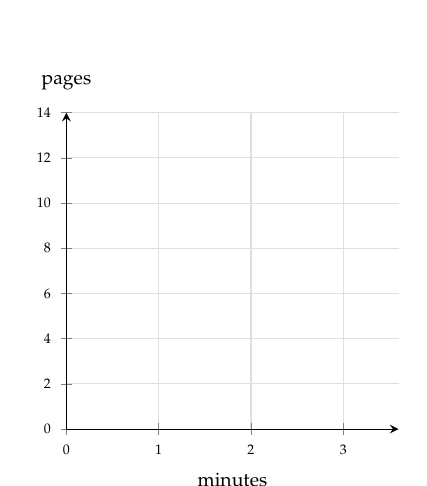
\begin{tikzpicture}
\begin{axis}[width=5.8cm,height=5.6cm,axis lines=left,xmin=0,xmax=3.6,ymin=0,ymax=14,xtick={0,...,3},ytick={0,2,...,14},
  grid=both,grid style={gray!25},xlabel={\scriptsize minutes},ylabel={\scriptsize pages},tick label style={font=\tiny},
  ylabel style={rotate=-90,at={(axis description cs:0,1.04)},anchor=south}]
\ifkey\addplot[FangBlue,thick,domain=0:3.3]{4*x};\addplot[only marks,mark=*,mark options={fill=FangBlue,draw=FangBlue}] coordinates{(0,0)(1,4)(2,8)(3,12)};\fi
\end{axis}
\end{tikzpicture}
\end{minipage}
\np[5.6cm]\item \begin{minipage}[t]{0.52\textwidth}\vspace{0pt}
Which graph shows a proportional relationship? For that one, find the constant of proportionality $k$.
\work[0.2cm]{Graph \textbf{B}: a straight line through the origin, through $(2,5)$, so $k=\tfrac52=2.5$. \ Graph A is a straight line but starts at $(0,2)$, so it is \textbf{not} proportional.}
\end{minipage}\hfill
\begin{minipage}[t]{0.44\textwidth}\vspace{0pt}\centering
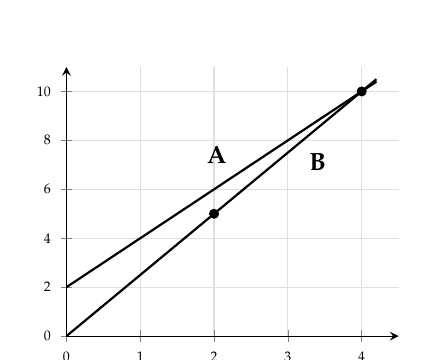
\begin{tikzpicture}
\begin{axis}[width=5.8cm,height=5cm,axis lines=left,xmin=0,xmax=4.5,ymin=0,ymax=11,xtick={0,...,4},ytick={0,2,...,10},
  grid=both,grid style={gray!25},tick label style={font=\tiny}]
\addplot[FangRed,thick,domain=0:4.2]{2*x+2} node[pos=0.55,above left,font=\small\bfseries]{A};
\addplot[FangBlue,thick,domain=0:4.2]{2.5*x} node[pos=0.75,below right,font=\small\bfseries]{B};
\addplot[only marks,mark=*,mark size=1.6pt,mark options={fill=FangBlue,draw=FangBlue}] coordinates{(2,5)(4,10)};
\end{axis}
\end{tikzpicture}
\end{minipage}
\np[3cm]\item \hard\ A proportional graph passes through $(6,\,15)$. Find $k$, write the equation, and find $y$ when $x=10$.
\work[1.6cm]{$k=\dfrac{15}{6}=2.5$. \ $y=2.5x$. \ When $x=10$: $y=25$. \ (Check: $(2,5)$ is also on the line, $5\div2=2.5$ \checkmark)}
\end{enumerate}

\needspace{5cm}{\large\bfseries\color{FangBlue}G.\ Challenge} \hard

\begin{enumerate}[resume,leftmargin=*,label=\textbf{\arabic*.},itemsep=6pt]
\np[3cm]\item Point $P(-3,\,a)$ is $7$ units from $Q(-3,\,2)$. Find \textbf{both} possible values of $a$.
\work[1.6cm]{Same $x$, so $|a-2|=7$: \ $a=2+7=9$ or $a=2-7=-5$. \ Points $(-3,9)$ and $(-3,-5)$.}
\np[3cm]\item The rectangle $(1,1)$, $(5,1)$, $(5,3)$, $(1,3)$ is reflected over the $y$-axis. List the new vertices. Did the area change?
\work[1.6cm]{$(-1,1)$, $(-5,1)$, $(-5,3)$, $(-1,3)$. The area stays $4\times2=8$ square units — a reflection flips the shape but does not change its size.}
\end{enumerate}

\ifkey\else
\vfill
\begin{simple}
\textbf{Before the test:} $x$ first, then $y$ \;·\; quadrants go counterclockwise from top right \;·\; across an axis, \textbf{add} distances \;·\; proportional = straight line \textbf{through the origin}, unit rate at $(1,k)$.
\end{simple}
\fi

\end{document}
"
% =====================================================================
\documentclass[12pt,letterpaper]{article}
\usepackage[margin=0.8in,top=0.85in,bottom=0.8in]{geometry}
\usepackage{mathpazo}
\usepackage[T1]{fontenc}
\usepackage{amsmath,amssymb}
\usepackage{xcolor}
\usepackage{enumitem}
\usepackage{multicol}
\usepackage{booktabs}
\usepackage{needspace}
\usepackage{fancyhdr}
\usepackage[most]{tcolorbox}
\usepackage{pgfplots}
\pgfplotsset{compat=1.17}
\usetikzlibrary{arrows.meta,calc}

\definecolor{FangBlue}{HTML}{000000}
\definecolor{FangTeal}{HTML}{000000}
\definecolor{FangGold}{HTML}{555555}
\definecolor{FangRed}{HTML}{000000}
\definecolor{FangGreen}{HTML}{000000}
\definecolor{FangPurple}{HTML}{000000}
\definecolor{Soft}{HTML}{FFFFFF}

\newif\ifkey
\ifdefined\iskey \keytrue \else \keyfalse \fi

\pagestyle{fancy}\fancyhf{}
\renewcommand{\headrulewidth}{0.4pt}
\fancyhead[L]{\small\color{FangBlue}\textbf{Prof. Fang Math} \,|\, Grade 7 \,·\, Graphing on the Coordinate Plane}
\fancyhead[R]{\small\ifkey\textcolor{FangRed}{\textbf{ANSWER KEY}}\else Name: \underline{\hspace{4.2cm}}\fi}
\fancyfoot[C]{\small\thepage}
\fancyfoot[R]{\scriptsize\color{gray}fangmath.com}
\setlength{\headheight}{14pt}
\setlength{\parindent}{0pt}
\setlength{\parskip}{4pt}

% ---------- boxes ----------
\newtcolorbox{idea}[1][]{colback=Soft,colframe=FangBlue,boxrule=0.8pt,arc=3pt,left=8pt,right=8pt,top=6pt,bottom=6pt,
  fonttitle=\bfseries,coltitle=white,colbacktitle=FangBlue,title={#1}}
\newtcolorbox{example}[1][]{colback=white,colframe=FangTeal,boxrule=0.6pt,arc=3pt,left=8pt,right=8pt,top=5pt,bottom=5pt,
  fonttitle=\bfseries,coltitle=FangTeal,colbacktitle=white,title={#1},attach boxed title to top left={xshift=8pt,yshift=-7pt},boxed title style={boxrule=0pt,colframe=white}, enhanced}
\newtcolorbox{warn}{colback=FangRed!5,colframe=FangRed,boxrule=0.6pt,arc=3pt,left=8pt,right=8pt,top=4pt,bottom=4pt,leftrule=3pt}
\newtcolorbox{simple}{colback=FangGold!10,colframe=FangGold,boxrule=0.6pt,arc=3pt,left=8pt,right=8pt,top=4pt,bottom=4pt,leftrule=3pt}
\newtcolorbox{sol}{colback=FangGreen!6,colframe=FangGreen,boxrule=0.5pt,arc=2pt,left=6pt,right=6pt,top=3pt,bottom=3pt,breakable}

\newcommand{\badge}[2]{\tcbox[on line,colback=#1,colframe=#1,coltext=white,boxrule=0pt,arc=6pt,left=4pt,right=4pt,top=1pt,bottom=1pt,fontupper=\scriptsize\bfseries]{#2}}
\newcommand{\easy}{\badge{FangGreen}{EASY}}
\newcommand{\medium}{\badge{FangTeal}{MEDIUM}}
\newcommand{\hard}{\badge{FangRed}{HARD}}
\newcommand{\work}[2][]{\ifkey\begin{sol}#2\end{sol}\else\vspace*{#1}\fi}
\newcommand{\np}[1][6cm]{\needspace{#1}}
\newcommand{\sect}[2]{\par\needspace{7cm}\medskip{\Large\bfseries\color{FangBlue}\tcbox[on line,colback=FangBlue,colframe=FangBlue,coltext=white,arc=2pt,boxrule=0pt,left=5pt,right=5pt,top=1pt,bottom=1pt]{#1}\ #2}\par\smallskip}

% ---------- right-triangle picture: \rt{scale}{a}{b}{labels...} ----------
% vertices: C = right angle at origin, A = (b,0) [the angle we look from], B = (0,a)
% ---------- coordinate grid: \cg[size]{xmin}{xmax}{ymin}{ymax}{plot commands} ----------
\newcommand{\cg}[6][5.4cm]{\begin{tikzpicture}\begin{axis}[width=#1,height=#1,axis lines=middle,
  xmin=#2-0.6,xmax=#3+0.6,ymin=#4-0.6,ymax=#5+0.6,xtick={#2,...,#3},ytick={#4,...,#5},
  grid=both,grid style={gray!28},xlabel={\scriptsize$x$},ylabel={\scriptsize$y$},
  tick label style={font=\tiny},axis line style={-{Stealth[length=4pt]},thick},clip=false,
  xticklabel style={fill=white,inner sep=1pt},yticklabel style={fill=white,inner sep=1pt}]#6\end{axis}\end{tikzpicture}}
\newcommand{\pt}[4][FangBlue]{\fill[#1](axis cs:#2,#3) circle(2.3pt) node[above right,font=\scriptsize\bfseries,text=#1,inner sep=1.5pt]{#4};}
\newcommand{\blank}{\underline{\hspace{1.6cm}}}

\begin{document}

% ======================= TITLE =======================
\begin{center}
{\color{FangBlue}\Huge\bfseries Graphing on the Coordinate Plane}\\[3pt]
{\large Test review: points, quadrants, reflections, distance, shapes and proportional graphs}
\ifkey\\[3pt]{\color{FangRed}\large\bfseries Answer Key}\fi
\end{center}
\vspace{-2pt}

% ======================= PART 1 =======================
\sect{1}{The coordinate plane}

\begin{minipage}[c]{0.46\textwidth}\centering
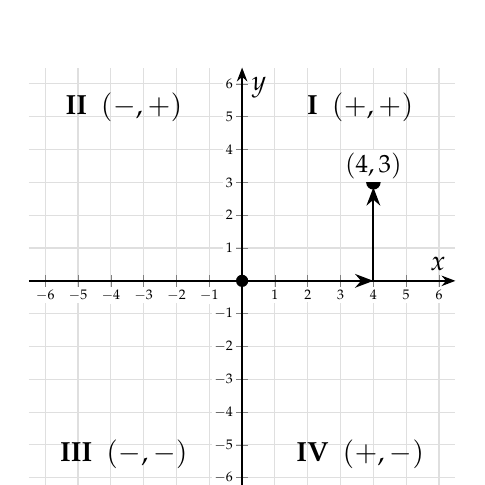
\begin{tikzpicture}
\begin{axis}[width=7cm,height=7cm,axis lines=middle,xmin=-6.5,xmax=6.5,ymin=-6.5,ymax=6.5,
  xtick={-6,...,6},ytick={-6,...,6},grid=both,grid style={gray!25},xlabel={$x$},ylabel={$y$},
  tick label style={font=\tiny},axis line style={-{Stealth[length=5pt]},thick},
  xticklabel style={fill=white,inner sep=1pt},yticklabel style={fill=white,inner sep=1pt}]
\node[FangTeal,font=\bfseries] at (axis cs:3.6,5.3) {I \ $(+,+)$};
\node[FangTeal,font=\bfseries] at (axis cs:-3.6,5.3) {II \ $(-,+)$};
\node[FangTeal,font=\bfseries] at (axis cs:-3.6,-5.3) {III \ $(-,-)$};
\node[FangTeal,font=\bfseries] at (axis cs:3.6,-5.3) {IV \ $(+,-)$};
\draw[FangRed,thick,-{Stealth}] (axis cs:0,0) -- (axis cs:4,0);
\draw[FangRed,thick,-{Stealth}] (axis cs:4,0) -- (axis cs:4,2.85);
\fill[FangRed](axis cs:4,3) circle(2.6pt) node[above,font=\small\bfseries,fill=white,inner sep=1pt]{$(4,3)$};
\fill(axis cs:0,0) circle(2.2pt);
\end{axis}
\end{tikzpicture}
\end{minipage}\hfill
\begin{minipage}[c]{0.52\textwidth}
\begin{itemize}[leftmargin=*,itemsep=3pt]
\item The \textbf{$x$-axis} goes left–right; the \textbf{$y$-axis} goes up–down. They cross at the \textbf{origin} $(0,0)$.
\item An \textbf{ordered pair} $(x,\,y)$: \textbf{first} walk left/right ($x$), \textbf{then} up/down ($y$). \\
\emph{“Walk to the elevator, then ride it.”}
\item The axes cut the plane into four \textbf{quadrants}, numbered I–IV \textbf{counterclockwise}, starting at the top right.
\item A point \textbf{on an axis} (like $(0,5)$ or $(-2,0)$) is in \textbf{no} quadrant.
\end{itemize}
\end{minipage}

\begin{warn}
\textbf{Watch out:} $(4,3)$ and $(3,4)$ are \textbf{different} points. Order matters: $x$ always comes first.
\end{warn}

% ======================= PART 2 =======================
\sect{2}{Reflections — flip over an axis}

\begin{minipage}[c]{0.46\textwidth}\centering
\cg[6.4cm]{-5}{5}{-5}{5}{
\pt[FangBlue]{3}{2}{$A(3,2)$}
\fill[FangRed](axis cs:3,-2) circle(2.3pt) node[below right,font=\scriptsize\bfseries,text=FangRed]{$(3,-2)$};
\fill[FangGreen](axis cs:-3,2) circle(2.3pt) node[above left,font=\scriptsize\bfseries,text=FangGreen]{$(-3,2)$};
\draw[FangRed,dashed](axis cs:3,2)--(axis cs:3,-2);
\draw[FangGreen,dashed](axis cs:3,2)--(axis cs:-3,2);}
\end{minipage}\hfill
\begin{minipage}[c]{0.52\textwidth}
\renewcommand{\arraystretch}{1.35}
\begin{tabular}{@{}lll@{}}
\toprule
\textbf{Reflect over\ldots} & \textbf{Rule} & \textbf{Example}\\ \midrule
\textcolor{FangRed}{the $x$-axis} & $(x,y)\to(x,\,-y)$ & $(3,2)\to(3,-2)$\\
\textcolor{FangGreen}{the $y$-axis} & $(x,y)\to(-x,\,y)$ & $(3,2)\to(-3,2)$\\
\bottomrule
\end{tabular}\par\medskip
\textbf{Memory trick:} over the \textbf{$x$-axis}, the \textbf{$x$ stays}; only $y$ changes sign. Over the \textbf{$y$-axis}, the \textbf{$y$ stays}.
\end{minipage}

% ======================= PART 3 =======================
\sect{3}{Distance between two points on a line}

\begin{idea}[Same $x$ or same $y$? Count — or use absolute value]
\textbf{Same quadrant / same side:} subtract. \quad $(2,5)$ to $(2,1)$: \ $5-1=4$ units.\par
\textbf{Opposite sides of an axis:} \textbf{add} the absolute values. \quad $(-3,4)$ to $(5,4)$: \ $|-3|+|5|=3+5=8$ units.\par
One rule for both: \textbf{distance} $=|\,\text{difference}\,|$. \quad $|5-(-3)|=|8|=8$. \ \ Distance is never negative.
\end{idea}

\begin{simple}
\textbf{Simple case first:} from $(-1,0)$ to $(1,0)$ — count the squares: $2$. And $|-1|+|1|=2$ \checkmark. That's why you \textbf{add} across the axis.
\end{simple}

% ======================= PART 4 =======================
\sect{4}{Shapes on the coordinate plane}

\begin{example}[Example \;·\; rectangle $ABCD$ with $A(-3,2)$, $B(4,2)$, $C(4,-1)$, $D(-3,-1)$]
\begin{minipage}[c]{0.4\textwidth}\centering
\cg[5.6cm]{-4}{5}{-2}{3}{
\draw[FangBlue,thick,fill=FangBlue!8](axis cs:-3,2)--(axis cs:4,2)--(axis cs:4,-1)--(axis cs:-3,-1)--cycle;
\pt{-3}{2}{A}\pt{4}{2}{B}\pt{4}{-1}{C}\pt{-3}{-1}{D}}
\end{minipage}\hfill
\begin{minipage}[c]{0.56\textwidth}
Length $AB$: same $y$, so $|4-(-3)|=7$. \\
Width $BC$: same $x$, so $|2-(-1)|=3$. \\[3pt]
\textbf{Perimeter} $=7+3+7+3=20$ units. \\
\textbf{Area} $=7\times3=21$ square units.
\end{minipage}
\end{example}

% ======================= PART 5 =======================
\sect{5}{Graphing a proportional relationship}

\begin{example}[Example \;·\; Tickets cost \$3 each]
\begin{minipage}[c]{0.42\textwidth}\centering
\begin{tabular}{c|ccccc}
tickets $x$ & 0 & 1 & 2 & 3 & 4\\ \hline
cost $y$ (\$) & 0 & 3 & 6 & 9 & 12
\end{tabular}\\[6pt]
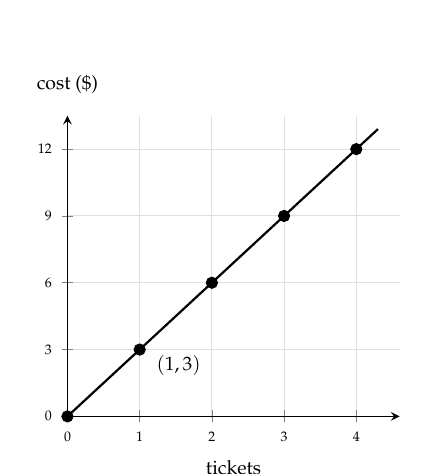
\begin{tikzpicture}
\begin{axis}[width=5.8cm,height=5.4cm,axis lines=left,xmin=0,xmax=4.6,ymin=0,ymax=13.5,xtick={0,...,4},ytick={0,3,...,12},
  grid=both,grid style={gray!25},xlabel={\scriptsize tickets},ylabel={\scriptsize cost (\$)},tick label style={font=\tiny},
  ylabel style={rotate=-90,at={(axis description cs:0,1.04)},anchor=south}]
\addplot[FangBlue,thick,domain=0:4.3]{3*x};
\addplot[only marks,mark=*,mark options={fill=FangBlue,draw=FangBlue}] coordinates{(0,0)(1,3)(2,6)(3,9)(4,12)};
\node[FangRed,font=\scriptsize\bfseries,anchor=west] at (axis cs:1.1,2.3) {$(1,3)$};
\end{axis}
\end{tikzpicture}
\end{minipage}\hfill
\begin{minipage}[c]{0.55\textwidth}
\textbf{How to tell it's proportional from a graph:}
\begin{enumerate}[leftmargin=*,itemsep=2pt]
\item the points are on a \textbf{straight line}, and
\item the line goes \textbf{through the origin} $(0,0)$.
\end{enumerate}
The \textbf{constant of proportionality} (unit rate) is $k=\dfrac{y}{x}=\dfrac{3}{1}=3$. Equation: $y=3x$.\par
\textbf{Look for the point $(1,\,k)$}: here $(1,3)$ means \emph{1 ticket costs \$3}.\par
A point like $(4,12)$ means \emph{4 tickets cost \$12}.
\end{minipage}
\end{example}

\begin{warn}
\textbf{Not proportional:} a straight line that \textbf{doesn't} pass through $(0,0)$ — for example a \$5 entry fee plus \$3 per ride: $y=3x+5$ starts at $(0,5)$.
\end{warn}

% ======================= PRACTICE =======================
\sect{6}{Practice}
\ifkey\else\textit{Show your work. Label every point you plot.}\fi

\needspace{8cm}{\large\bfseries\color{FangBlue}A.\ Read and plot points} \easy

\begin{minipage}[t]{0.42\textwidth}\vspace{0pt}\centering
\cg[6.2cm]{-6}{6}{-6}{6}{
\pt{2}{5}{A}\pt{-4}{3}{B}\pt{-3}{-2}{C}\pt{5}{-4}{D}\pt{0}{-5}{E}\pt{-6}{0}{F}
\ifkey
\pt[FangRed]{3}{1}{P}\pt[FangRed]{-5}{-4}{Q}\pt[FangRed]{0}{4}{R}\pt[FangRed]{4}{-2}{S}
\fi}
\end{minipage}\hfill
\begin{minipage}[t]{0.55\textwidth}\vspace{2pt}
\begin{enumerate}[leftmargin=*,label=\textbf{\arabic*.},itemsep=5pt]
\item Write the coordinates of each point.\\[3pt]
$A$ \ifkey\textcolor{FangGreen}{$(2,5)$}\else\blank\fi \quad $B$ \ifkey\textcolor{FangGreen}{$(-4,3)$}\else\blank\fi \\[3pt]
$C$ \ifkey\textcolor{FangGreen}{$(-3,-2)$}\else\blank\fi \quad $D$ \ifkey\textcolor{FangGreen}{$(5,-4)$}\else\blank\fi \\[3pt]
$E$ \ifkey\textcolor{FangGreen}{$(0,-5)$}\else\blank\fi \quad $F$ \ifkey\textcolor{FangGreen}{$(-6,0)$}\else\blank\fi
\item Which quadrant is each of $A$, $B$, $C$, $D$ in? Which points are on an axis?
\work[1.2cm]{$A$: I, \ $B$: II, \ $C$: III, \ $D$: IV. \ $E$ and $F$ are on an axis (no quadrant).}
\item Plot and label on the same grid: \\ $P(3,1)$, \ $Q(-5,-4)$, \ $R(0,4)$, \ $S(4,-2)$.
\work[0.4cm]{Points $P$, $Q$, $R$, $S$ are plotted on the grid.}
\end{enumerate}
\end{minipage}

\needspace{5cm}{\large\bfseries\color{FangBlue}B.\ Signs and quadrants} \easy\ \medium

\begin{enumerate}[start=4,leftmargin=*,label=\textbf{\arabic*.},itemsep=5pt]
\np[2cm]\item Name the quadrant: \quad (a) $(-7,\,2)$ \quad (b) $(6,\,-1)$ \quad (c) $(-0.5,\,-8)$ \quad (d) $(3\tfrac12,\,4)$
\work[1cm]{(a) II \quad (b) IV \quad (c) III \quad (d) I}
\np[2cm]\item A point has a negative $x$-coordinate and a positive $y$-coordinate. Which quadrant is it in?
\work[1cm]{Quadrant II \ $(-,+)$.}
\np[2cm]\item True or false: the point $(0,-3)$ is in Quadrant IV. Explain.
\work[1.2cm]{False. Its $x$-coordinate is $0$, so it lies \textbf{on the $y$-axis} — in no quadrant.}
\end{enumerate}

\needspace{5cm}{\large\bfseries\color{FangBlue}C.\ Reflections} \medium

\begin{enumerate}[resume,leftmargin=*,label=\textbf{\arabic*.},itemsep=5pt]
\np[2cm]\item Reflect $(5,-2)$ over the $x$-axis. \quad Then reflect $(5,-2)$ over the $y$-axis.
\work[1cm]{Over the $x$-axis: $(5,2)$. \quad Over the $y$-axis: $(-5,-2)$.}
\np[2cm]\item $(-4,\,6)$ is reflected over the $y$-axis, and then the new point is reflected over the $x$-axis. Where does it end up? Which quadrant?
\work[1.4cm]{$(-4,6)\to(4,6)\to(4,-6)$. \ Quadrant IV. (Two flips change both signs.)}
\np[2cm]\item Point $M$ is $(a,\,b)$ and point $N$ is $(a,\,-b)$. Over which axis is $N$ the reflection of $M$?
\work[1cm]{The $x$-axis (the $x$-coordinate stayed the same).}
\end{enumerate}

\needspace{5cm}{\large\bfseries\color{FangBlue}D.\ Distance} \medium

\begin{enumerate}[resume,leftmargin=*,label=\textbf{\arabic*.},itemsep=5pt]
\np[2cm]\item Find the distance between $(3,\,7)$ and $(3,\,-2)$.
\work[1.2cm]{Same $x$. Opposite sides of the $x$-axis: $7+2=9$ units. \ (Or $|7-(-2)|=9$.)}
\np[2cm]\item Find the distance between $(-6,\,-1)$ and $(-2,\,-1)$.
\work[1.2cm]{Same $y$. Same side: $|-2-(-6)|=|4|=4$ units.}
\np[2cm]\item Point $A$ is at $(-5,\,4)$. Point $B$ is $9$ units to the right of $A$. Find $B$. Which quadrant is $B$ in?
\work[1.2cm]{$B=(-5+9,\,4)=(4,4)$, \ Quadrant I.}
\np[2.4cm]\item A diver is at $-12$ m and a seagull is at $+15$ m, straight above the diver. How far apart are they?
\work[1.2cm]{$|-12|+|15|=12+15=27$ m (opposite sides of sea level, so add).}
\end{enumerate}

\needspace{7cm}{\large\bfseries\color{FangBlue}E.\ Shapes} \medium\ \hard

\begin{enumerate}[resume,leftmargin=*,label=\textbf{\arabic*.},itemsep=6pt]
\np[5cm]\item \begin{minipage}[t]{0.5\textwidth}\vspace{0pt}
Plot $J(-4,3)$, $K(2,3)$, $L(2,-2)$ and $M(-4,-2)$ and connect them in order. \\
(a) What shape is $JKLM$? \\ (b) Find its perimeter. \\ (c) Find its area.
\work[0.2cm]{(a) A rectangle. \ (b) $JK=|2-(-4)|=6$, $KL=|3-(-2)|=5$. Perimeter $=2(6+5)=22$ units. \ (c) Area $=6\times5=30$ square units.}
\end{minipage}\hfill
\begin{minipage}[t]{0.42\textwidth}\vspace{0pt}\centering
\cg[5.6cm]{-5}{5}{-5}{5}{\ifkey\draw[FangBlue,thick,fill=FangBlue!8](axis cs:-4,3)--(axis cs:2,3)--(axis cs:2,-2)--(axis cs:-4,-2)--cycle;\pt{-4}{3}{J}\pt{2}{3}{K}\pt{2}{-2}{L}\pt{-4}{-2}{M}\fi}
\end{minipage}
\np[2.6cm]\item Three corners of a square are $(-1,4)$, $(3,4)$ and $(3,0)$. Find the fourth corner and the area of the square.
\work[1.4cm]{The fourth corner is $(-1,0)$. Side $=|3-(-1)|=4$, so area $=4\times4=16$ square units.}
\np[3cm]\item \hard\ A triangle has vertices $(-2,-3)$, $(4,-3)$ and $(1,5)$. Find its area.
\work[1.6cm]{Base on $y=-3$: $|4-(-2)|=6$. Height: from $y=-3$ up to $y=5$ is $|5-(-3)|=8$. \ Area $=\tfrac12\cdot6\cdot8=24$ square units.}
\end{enumerate}

\needspace{8cm}{\large\bfseries\color{FangBlue}F.\ Proportional relationships} \medium\ \hard

\begin{enumerate}[resume,leftmargin=*,label=\textbf{\arabic*.},itemsep=6pt]
\np[6.5cm]\item \begin{minipage}[t]{0.52\textwidth}\vspace{0pt}
A printer prints $4$ pages per minute. \\[2pt]
\begin{tabular}{c|cccc}minutes $x$ & 0 & 1 & 2 & 3\\ \hline pages $y$ & \ifkey 0\else\fi & \ifkey 4\else\fi & \ifkey 8\else\fi & \ifkey 12\else\fi\end{tabular}\\[4pt]
(a) Complete the table and graph it. \\
(b) Is the relationship proportional? How can you tell from the graph? \\
(c) Write an equation. \quad (d) What does the point $(1,4)$ mean?
\work[0.2cm]{(b) Yes — the points make a straight line through $(0,0)$. \ (c) $y=4x$. \ (d) In $1$ minute the printer prints $4$ pages (the unit rate).}
\end{minipage}\hfill
\begin{minipage}[t]{0.44\textwidth}\vspace{0pt}\centering
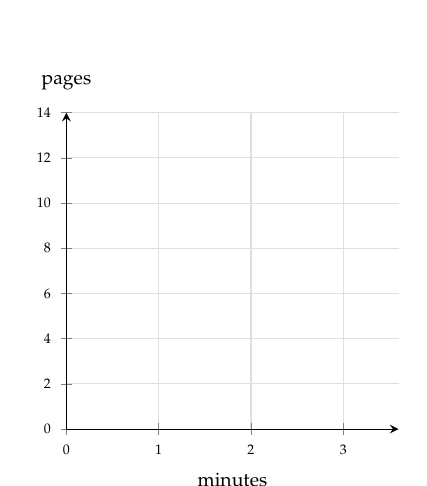
\begin{tikzpicture}
\begin{axis}[width=5.8cm,height=5.6cm,axis lines=left,xmin=0,xmax=3.6,ymin=0,ymax=14,xtick={0,...,3},ytick={0,2,...,14},
  grid=both,grid style={gray!25},xlabel={\scriptsize minutes},ylabel={\scriptsize pages},tick label style={font=\tiny},
  ylabel style={rotate=-90,at={(axis description cs:0,1.04)},anchor=south}]
\ifkey\addplot[FangBlue,thick,domain=0:3.3]{4*x};\addplot[only marks,mark=*,mark options={fill=FangBlue,draw=FangBlue}] coordinates{(0,0)(1,4)(2,8)(3,12)};\fi
\end{axis}
\end{tikzpicture}
\end{minipage}
\np[5.6cm]\item \begin{minipage}[t]{0.52\textwidth}\vspace{0pt}
Which graph shows a proportional relationship? For that one, find the constant of proportionality $k$.
\work[0.2cm]{Graph \textbf{B}: a straight line through the origin, through $(2,5)$, so $k=\tfrac52=2.5$. \ Graph A is a straight line but starts at $(0,2)$, so it is \textbf{not} proportional.}
\end{minipage}\hfill
\begin{minipage}[t]{0.44\textwidth}\vspace{0pt}\centering
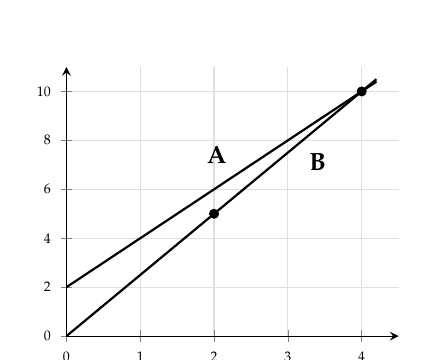
\begin{tikzpicture}
\begin{axis}[width=5.8cm,height=5cm,axis lines=left,xmin=0,xmax=4.5,ymin=0,ymax=11,xtick={0,...,4},ytick={0,2,...,10},
  grid=both,grid style={gray!25},tick label style={font=\tiny}]
\addplot[FangRed,thick,domain=0:4.2]{2*x+2} node[pos=0.55,above left,font=\small\bfseries]{A};
\addplot[FangBlue,thick,domain=0:4.2]{2.5*x} node[pos=0.75,below right,font=\small\bfseries]{B};
\addplot[only marks,mark=*,mark size=1.6pt,mark options={fill=FangBlue,draw=FangBlue}] coordinates{(2,5)(4,10)};
\end{axis}
\end{tikzpicture}
\end{minipage}
\np[3cm]\item \hard\ A proportional graph passes through $(6,\,15)$. Find $k$, write the equation, and find $y$ when $x=10$.
\work[1.6cm]{$k=\dfrac{15}{6}=2.5$. \ $y=2.5x$. \ When $x=10$: $y=25$. \ (Check: $(2,5)$ is also on the line, $5\div2=2.5$ \checkmark)}
\end{enumerate}

\needspace{5cm}{\large\bfseries\color{FangBlue}G.\ Challenge} \hard

\begin{enumerate}[resume,leftmargin=*,label=\textbf{\arabic*.},itemsep=6pt]
\np[3cm]\item Point $P(-3,\,a)$ is $7$ units from $Q(-3,\,2)$. Find \textbf{both} possible values of $a$.
\work[1.6cm]{Same $x$, so $|a-2|=7$: \ $a=2+7=9$ or $a=2-7=-5$. \ Points $(-3,9)$ and $(-3,-5)$.}
\np[3cm]\item The rectangle $(1,1)$, $(5,1)$, $(5,3)$, $(1,3)$ is reflected over the $y$-axis. List the new vertices. Did the area change?
\work[1.6cm]{$(-1,1)$, $(-5,1)$, $(-5,3)$, $(-1,3)$. The area stays $4\times2=8$ square units — a reflection flips the shape but does not change its size.}
\end{enumerate}

\ifkey\else
\vfill
\begin{simple}
\textbf{Before the test:} $x$ first, then $y$ \;·\; quadrants go counterclockwise from top right \;·\; across an axis, \textbf{add} distances \;·\; proportional = straight line \textbf{through the origin}, unit rate at $(1,k)$.
\end{simple}
\fi

\end{document}
"
% =====================================================================
\documentclass[12pt,letterpaper]{article}
\usepackage[margin=0.8in,top=0.85in,bottom=0.8in]{geometry}
\usepackage{mathpazo}
\usepackage[T1]{fontenc}
\usepackage{amsmath,amssymb}
\usepackage{xcolor}
\usepackage{enumitem}
\usepackage{multicol}
\usepackage{booktabs}
\usepackage{needspace}
\usepackage{fancyhdr}
\usepackage[most]{tcolorbox}
\usepackage{pgfplots}
\pgfplotsset{compat=1.17}
\usetikzlibrary{arrows.meta,calc}

\definecolor{FangBlue}{HTML}{000000}
\definecolor{FangTeal}{HTML}{000000}
\definecolor{FangGold}{HTML}{555555}
\definecolor{FangRed}{HTML}{000000}
\definecolor{FangGreen}{HTML}{000000}
\definecolor{FangPurple}{HTML}{000000}
\definecolor{Soft}{HTML}{FFFFFF}

\newif\ifkey
\ifdefined\iskey \keytrue \else \keyfalse \fi

\pagestyle{fancy}\fancyhf{}
\renewcommand{\headrulewidth}{0.4pt}
\fancyhead[L]{\small\color{FangBlue}\textbf{Prof. Fang Math} \,|\, Grade 7 \,·\, Graphing on the Coordinate Plane}
\fancyhead[R]{\small\ifkey\textcolor{FangRed}{\textbf{ANSWER KEY}}\else Name: \underline{\hspace{4.2cm}}\fi}
\fancyfoot[C]{\small\thepage}
\fancyfoot[R]{\scriptsize\color{gray}fangmath.com}
\setlength{\headheight}{14pt}
\setlength{\parindent}{0pt}
\setlength{\parskip}{4pt}

% ---------- boxes ----------
\newtcolorbox{idea}[1][]{colback=Soft,colframe=FangBlue,boxrule=0.8pt,arc=3pt,left=8pt,right=8pt,top=6pt,bottom=6pt,
  fonttitle=\bfseries,coltitle=white,colbacktitle=FangBlue,title={#1}}
\newtcolorbox{example}[1][]{colback=white,colframe=FangTeal,boxrule=0.6pt,arc=3pt,left=8pt,right=8pt,top=5pt,bottom=5pt,
  fonttitle=\bfseries,coltitle=FangTeal,colbacktitle=white,title={#1},attach boxed title to top left={xshift=8pt,yshift=-7pt},boxed title style={boxrule=0pt,colframe=white}, enhanced}
\newtcolorbox{warn}{colback=FangRed!5,colframe=FangRed,boxrule=0.6pt,arc=3pt,left=8pt,right=8pt,top=4pt,bottom=4pt,leftrule=3pt}
\newtcolorbox{simple}{colback=FangGold!10,colframe=FangGold,boxrule=0.6pt,arc=3pt,left=8pt,right=8pt,top=4pt,bottom=4pt,leftrule=3pt}
\newtcolorbox{sol}{colback=FangGreen!6,colframe=FangGreen,boxrule=0.5pt,arc=2pt,left=6pt,right=6pt,top=3pt,bottom=3pt,breakable}

\newcommand{\badge}[2]{\tcbox[on line,colback=#1,colframe=#1,coltext=white,boxrule=0pt,arc=6pt,left=4pt,right=4pt,top=1pt,bottom=1pt,fontupper=\scriptsize\bfseries]{#2}}
\newcommand{\easy}{\badge{FangGreen}{EASY}}
\newcommand{\medium}{\badge{FangTeal}{MEDIUM}}
\newcommand{\hard}{\badge{FangRed}{HARD}}
\newcommand{\work}[2][]{\ifkey\begin{sol}#2\end{sol}\else\vspace*{#1}\fi}
\newcommand{\np}[1][6cm]{\needspace{#1}}
\newcommand{\sect}[2]{\par\needspace{7cm}\medskip{\Large\bfseries\color{FangBlue}\tcbox[on line,colback=FangBlue,colframe=FangBlue,coltext=white,arc=2pt,boxrule=0pt,left=5pt,right=5pt,top=1pt,bottom=1pt]{#1}\ #2}\par\smallskip}

% ---------- right-triangle picture: \rt{scale}{a}{b}{labels...} ----------
% vertices: C = right angle at origin, A = (b,0) [the angle we look from], B = (0,a)
% ---------- coordinate grid: \cg[size]{xmin}{xmax}{ymin}{ymax}{plot commands} ----------
\newcommand{\cg}[6][5.4cm]{\begin{tikzpicture}\begin{axis}[width=#1,height=#1,axis lines=middle,
  xmin=#2-0.6,xmax=#3+0.6,ymin=#4-0.6,ymax=#5+0.6,xtick={#2,...,#3},ytick={#4,...,#5},
  grid=both,grid style={gray!28},xlabel={\scriptsize$x$},ylabel={\scriptsize$y$},
  tick label style={font=\tiny},axis line style={-{Stealth[length=4pt]},thick},clip=false,
  xticklabel style={fill=white,inner sep=1pt},yticklabel style={fill=white,inner sep=1pt}]#6\end{axis}\end{tikzpicture}}
\newcommand{\pt}[4][FangBlue]{\fill[#1](axis cs:#2,#3) circle(2.3pt) node[above right,font=\scriptsize\bfseries,text=#1,inner sep=1.5pt]{#4};}
\newcommand{\blank}{\underline{\hspace{1.6cm}}}

\begin{document}

% ======================= TITLE =======================
\begin{center}
{\color{FangBlue}\Huge\bfseries Graphing on the Coordinate Plane}\\[3pt]
{\large Test review: points, quadrants, reflections, distance, shapes and proportional graphs}
\ifkey\\[3pt]{\color{FangRed}\large\bfseries Answer Key}\fi
\end{center}
\vspace{-2pt}

% ======================= PART 1 =======================
\sect{1}{The coordinate plane}

\begin{minipage}[c]{0.46\textwidth}\centering
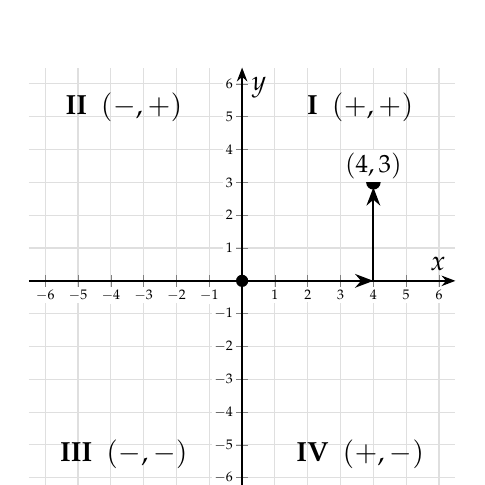
\begin{tikzpicture}
\begin{axis}[width=7cm,height=7cm,axis lines=middle,xmin=-6.5,xmax=6.5,ymin=-6.5,ymax=6.5,
  xtick={-6,...,6},ytick={-6,...,6},grid=both,grid style={gray!25},xlabel={$x$},ylabel={$y$},
  tick label style={font=\tiny},axis line style={-{Stealth[length=5pt]},thick},
  xticklabel style={fill=white,inner sep=1pt},yticklabel style={fill=white,inner sep=1pt}]
\node[FangTeal,font=\bfseries] at (axis cs:3.6,5.3) {I \ $(+,+)$};
\node[FangTeal,font=\bfseries] at (axis cs:-3.6,5.3) {II \ $(-,+)$};
\node[FangTeal,font=\bfseries] at (axis cs:-3.6,-5.3) {III \ $(-,-)$};
\node[FangTeal,font=\bfseries] at (axis cs:3.6,-5.3) {IV \ $(+,-)$};
\draw[FangRed,thick,-{Stealth}] (axis cs:0,0) -- (axis cs:4,0);
\draw[FangRed,thick,-{Stealth}] (axis cs:4,0) -- (axis cs:4,2.85);
\fill[FangRed](axis cs:4,3) circle(2.6pt) node[above,font=\small\bfseries,fill=white,inner sep=1pt]{$(4,3)$};
\fill(axis cs:0,0) circle(2.2pt);
\end{axis}
\end{tikzpicture}
\end{minipage}\hfill
\begin{minipage}[c]{0.52\textwidth}
\begin{itemize}[leftmargin=*,itemsep=3pt]
\item The \textbf{$x$-axis} goes left–right; the \textbf{$y$-axis} goes up–down. They cross at the \textbf{origin} $(0,0)$.
\item An \textbf{ordered pair} $(x,\,y)$: \textbf{first} walk left/right ($x$), \textbf{then} up/down ($y$). \\
\emph{“Walk to the elevator, then ride it.”}
\item The axes cut the plane into four \textbf{quadrants}, numbered I–IV \textbf{counterclockwise}, starting at the top right.
\item A point \textbf{on an axis} (like $(0,5)$ or $(-2,0)$) is in \textbf{no} quadrant.
\end{itemize}
\end{minipage}

\begin{warn}
\textbf{Watch out:} $(4,3)$ and $(3,4)$ are \textbf{different} points. Order matters: $x$ always comes first.
\end{warn}

% ======================= PART 2 =======================
\sect{2}{Reflections — flip over an axis}

\begin{minipage}[c]{0.46\textwidth}\centering
\cg[6.4cm]{-5}{5}{-5}{5}{
\pt[FangBlue]{3}{2}{$A(3,2)$}
\fill[FangRed](axis cs:3,-2) circle(2.3pt) node[below right,font=\scriptsize\bfseries,text=FangRed]{$(3,-2)$};
\fill[FangGreen](axis cs:-3,2) circle(2.3pt) node[above left,font=\scriptsize\bfseries,text=FangGreen]{$(-3,2)$};
\draw[FangRed,dashed](axis cs:3,2)--(axis cs:3,-2);
\draw[FangGreen,dashed](axis cs:3,2)--(axis cs:-3,2);}
\end{minipage}\hfill
\begin{minipage}[c]{0.52\textwidth}
\renewcommand{\arraystretch}{1.35}
\begin{tabular}{@{}lll@{}}
\toprule
\textbf{Reflect over\ldots} & \textbf{Rule} & \textbf{Example}\\ \midrule
\textcolor{FangRed}{the $x$-axis} & $(x,y)\to(x,\,-y)$ & $(3,2)\to(3,-2)$\\
\textcolor{FangGreen}{the $y$-axis} & $(x,y)\to(-x,\,y)$ & $(3,2)\to(-3,2)$\\
\bottomrule
\end{tabular}\par\medskip
\textbf{Memory trick:} over the \textbf{$x$-axis}, the \textbf{$x$ stays}; only $y$ changes sign. Over the \textbf{$y$-axis}, the \textbf{$y$ stays}.
\end{minipage}

% ======================= PART 3 =======================
\sect{3}{Distance between two points on a line}

\begin{idea}[Same $x$ or same $y$? Count — or use absolute value]
\textbf{Same quadrant / same side:} subtract. \quad $(2,5)$ to $(2,1)$: \ $5-1=4$ units.\par
\textbf{Opposite sides of an axis:} \textbf{add} the absolute values. \quad $(-3,4)$ to $(5,4)$: \ $|-3|+|5|=3+5=8$ units.\par
One rule for both: \textbf{distance} $=|\,\text{difference}\,|$. \quad $|5-(-3)|=|8|=8$. \ \ Distance is never negative.
\end{idea}

\begin{simple}
\textbf{Simple case first:} from $(-1,0)$ to $(1,0)$ — count the squares: $2$. And $|-1|+|1|=2$ \checkmark. That's why you \textbf{add} across the axis.
\end{simple}

% ======================= PART 4 =======================
\sect{4}{Shapes on the coordinate plane}

\begin{example}[Example \;·\; rectangle $ABCD$ with $A(-3,2)$, $B(4,2)$, $C(4,-1)$, $D(-3,-1)$]
\begin{minipage}[c]{0.4\textwidth}\centering
\cg[5.6cm]{-4}{5}{-2}{3}{
\draw[FangBlue,thick,fill=FangBlue!8](axis cs:-3,2)--(axis cs:4,2)--(axis cs:4,-1)--(axis cs:-3,-1)--cycle;
\pt{-3}{2}{A}\pt{4}{2}{B}\pt{4}{-1}{C}\pt{-3}{-1}{D}}
\end{minipage}\hfill
\begin{minipage}[c]{0.56\textwidth}
Length $AB$: same $y$, so $|4-(-3)|=7$. \\
Width $BC$: same $x$, so $|2-(-1)|=3$. \\[3pt]
\textbf{Perimeter} $=7+3+7+3=20$ units. \\
\textbf{Area} $=7\times3=21$ square units.
\end{minipage}
\end{example}

% ======================= PART 5 =======================
\sect{5}{Graphing a proportional relationship}

\begin{example}[Example \;·\; Tickets cost \$3 each]
\begin{minipage}[c]{0.42\textwidth}\centering
\begin{tabular}{c|ccccc}
tickets $x$ & 0 & 1 & 2 & 3 & 4\\ \hline
cost $y$ (\$) & 0 & 3 & 6 & 9 & 12
\end{tabular}\\[6pt]
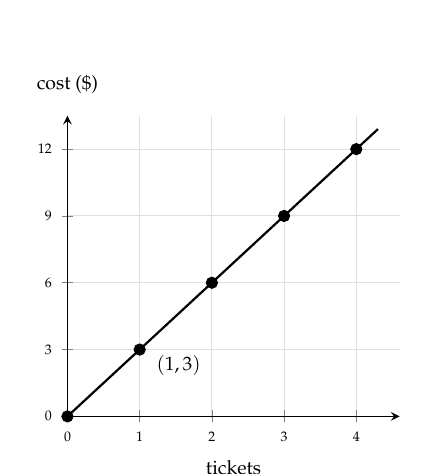
\begin{tikzpicture}
\begin{axis}[width=5.8cm,height=5.4cm,axis lines=left,xmin=0,xmax=4.6,ymin=0,ymax=13.5,xtick={0,...,4},ytick={0,3,...,12},
  grid=both,grid style={gray!25},xlabel={\scriptsize tickets},ylabel={\scriptsize cost (\$)},tick label style={font=\tiny},
  ylabel style={rotate=-90,at={(axis description cs:0,1.04)},anchor=south}]
\addplot[FangBlue,thick,domain=0:4.3]{3*x};
\addplot[only marks,mark=*,mark options={fill=FangBlue,draw=FangBlue}] coordinates{(0,0)(1,3)(2,6)(3,9)(4,12)};
\node[FangRed,font=\scriptsize\bfseries,anchor=west] at (axis cs:1.1,2.3) {$(1,3)$};
\end{axis}
\end{tikzpicture}
\end{minipage}\hfill
\begin{minipage}[c]{0.55\textwidth}
\textbf{How to tell it's proportional from a graph:}
\begin{enumerate}[leftmargin=*,itemsep=2pt]
\item the points are on a \textbf{straight line}, and
\item the line goes \textbf{through the origin} $(0,0)$.
\end{enumerate}
The \textbf{constant of proportionality} (unit rate) is $k=\dfrac{y}{x}=\dfrac{3}{1}=3$. Equation: $y=3x$.\par
\textbf{Look for the point $(1,\,k)$}: here $(1,3)$ means \emph{1 ticket costs \$3}.\par
A point like $(4,12)$ means \emph{4 tickets cost \$12}.
\end{minipage}
\end{example}

\begin{warn}
\textbf{Not proportional:} a straight line that \textbf{doesn't} pass through $(0,0)$ — for example a \$5 entry fee plus \$3 per ride: $y=3x+5$ starts at $(0,5)$.
\end{warn}

% ======================= PRACTICE =======================
\sect{6}{Practice}
\ifkey\else\textit{Show your work. Label every point you plot.}\fi

\needspace{8cm}{\large\bfseries\color{FangBlue}A.\ Read and plot points} \easy

\begin{minipage}[t]{0.42\textwidth}\vspace{0pt}\centering
\cg[6.2cm]{-6}{6}{-6}{6}{
\pt{2}{5}{A}\pt{-4}{3}{B}\pt{-3}{-2}{C}\pt{5}{-4}{D}\pt{0}{-5}{E}\pt{-6}{0}{F}
\ifkey
\pt[FangRed]{3}{1}{P}\pt[FangRed]{-5}{-4}{Q}\pt[FangRed]{0}{4}{R}\pt[FangRed]{4}{-2}{S}
\fi}
\end{minipage}\hfill
\begin{minipage}[t]{0.55\textwidth}\vspace{2pt}
\begin{enumerate}[leftmargin=*,label=\textbf{\arabic*.},itemsep=5pt]
\item Write the coordinates of each point.\\[3pt]
$A$ \ifkey\textcolor{FangGreen}{$(2,5)$}\else\blank\fi \quad $B$ \ifkey\textcolor{FangGreen}{$(-4,3)$}\else\blank\fi \\[3pt]
$C$ \ifkey\textcolor{FangGreen}{$(-3,-2)$}\else\blank\fi \quad $D$ \ifkey\textcolor{FangGreen}{$(5,-4)$}\else\blank\fi \\[3pt]
$E$ \ifkey\textcolor{FangGreen}{$(0,-5)$}\else\blank\fi \quad $F$ \ifkey\textcolor{FangGreen}{$(-6,0)$}\else\blank\fi
\item Which quadrant is each of $A$, $B$, $C$, $D$ in? Which points are on an axis?
\work[1.2cm]{$A$: I, \ $B$: II, \ $C$: III, \ $D$: IV. \ $E$ and $F$ are on an axis (no quadrant).}
\item Plot and label on the same grid: \\ $P(3,1)$, \ $Q(-5,-4)$, \ $R(0,4)$, \ $S(4,-2)$.
\work[0.4cm]{Points $P$, $Q$, $R$, $S$ are plotted on the grid.}
\end{enumerate}
\end{minipage}

\needspace{5cm}{\large\bfseries\color{FangBlue}B.\ Signs and quadrants} \easy\ \medium

\begin{enumerate}[start=4,leftmargin=*,label=\textbf{\arabic*.},itemsep=5pt]
\np[2cm]\item Name the quadrant: \quad (a) $(-7,\,2)$ \quad (b) $(6,\,-1)$ \quad (c) $(-0.5,\,-8)$ \quad (d) $(3\tfrac12,\,4)$
\work[1cm]{(a) II \quad (b) IV \quad (c) III \quad (d) I}
\np[2cm]\item A point has a negative $x$-coordinate and a positive $y$-coordinate. Which quadrant is it in?
\work[1cm]{Quadrant II \ $(-,+)$.}
\np[2cm]\item True or false: the point $(0,-3)$ is in Quadrant IV. Explain.
\work[1.2cm]{False. Its $x$-coordinate is $0$, so it lies \textbf{on the $y$-axis} — in no quadrant.}
\end{enumerate}

\needspace{5cm}{\large\bfseries\color{FangBlue}C.\ Reflections} \medium

\begin{enumerate}[resume,leftmargin=*,label=\textbf{\arabic*.},itemsep=5pt]
\np[2cm]\item Reflect $(5,-2)$ over the $x$-axis. \quad Then reflect $(5,-2)$ over the $y$-axis.
\work[1cm]{Over the $x$-axis: $(5,2)$. \quad Over the $y$-axis: $(-5,-2)$.}
\np[2cm]\item $(-4,\,6)$ is reflected over the $y$-axis, and then the new point is reflected over the $x$-axis. Where does it end up? Which quadrant?
\work[1.4cm]{$(-4,6)\to(4,6)\to(4,-6)$. \ Quadrant IV. (Two flips change both signs.)}
\np[2cm]\item Point $M$ is $(a,\,b)$ and point $N$ is $(a,\,-b)$. Over which axis is $N$ the reflection of $M$?
\work[1cm]{The $x$-axis (the $x$-coordinate stayed the same).}
\end{enumerate}

\needspace{5cm}{\large\bfseries\color{FangBlue}D.\ Distance} \medium

\begin{enumerate}[resume,leftmargin=*,label=\textbf{\arabic*.},itemsep=5pt]
\np[2cm]\item Find the distance between $(3,\,7)$ and $(3,\,-2)$.
\work[1.2cm]{Same $x$. Opposite sides of the $x$-axis: $7+2=9$ units. \ (Or $|7-(-2)|=9$.)}
\np[2cm]\item Find the distance between $(-6,\,-1)$ and $(-2,\,-1)$.
\work[1.2cm]{Same $y$. Same side: $|-2-(-6)|=|4|=4$ units.}
\np[2cm]\item Point $A$ is at $(-5,\,4)$. Point $B$ is $9$ units to the right of $A$. Find $B$. Which quadrant is $B$ in?
\work[1.2cm]{$B=(-5+9,\,4)=(4,4)$, \ Quadrant I.}
\np[2.4cm]\item A diver is at $-12$ m and a seagull is at $+15$ m, straight above the diver. How far apart are they?
\work[1.2cm]{$|-12|+|15|=12+15=27$ m (opposite sides of sea level, so add).}
\end{enumerate}

\needspace{7cm}{\large\bfseries\color{FangBlue}E.\ Shapes} \medium\ \hard

\begin{enumerate}[resume,leftmargin=*,label=\textbf{\arabic*.},itemsep=6pt]
\np[5cm]\item \begin{minipage}[t]{0.5\textwidth}\vspace{0pt}
Plot $J(-4,3)$, $K(2,3)$, $L(2,-2)$ and $M(-4,-2)$ and connect them in order. \\
(a) What shape is $JKLM$? \\ (b) Find its perimeter. \\ (c) Find its area.
\work[0.2cm]{(a) A rectangle. \ (b) $JK=|2-(-4)|=6$, $KL=|3-(-2)|=5$. Perimeter $=2(6+5)=22$ units. \ (c) Area $=6\times5=30$ square units.}
\end{minipage}\hfill
\begin{minipage}[t]{0.42\textwidth}\vspace{0pt}\centering
\cg[5.6cm]{-5}{5}{-5}{5}{\ifkey\draw[FangBlue,thick,fill=FangBlue!8](axis cs:-4,3)--(axis cs:2,3)--(axis cs:2,-2)--(axis cs:-4,-2)--cycle;\pt{-4}{3}{J}\pt{2}{3}{K}\pt{2}{-2}{L}\pt{-4}{-2}{M}\fi}
\end{minipage}
\np[2.6cm]\item Three corners of a square are $(-1,4)$, $(3,4)$ and $(3,0)$. Find the fourth corner and the area of the square.
\work[1.4cm]{The fourth corner is $(-1,0)$. Side $=|3-(-1)|=4$, so area $=4\times4=16$ square units.}
\np[3cm]\item \hard\ A triangle has vertices $(-2,-3)$, $(4,-3)$ and $(1,5)$. Find its area.
\work[1.6cm]{Base on $y=-3$: $|4-(-2)|=6$. Height: from $y=-3$ up to $y=5$ is $|5-(-3)|=8$. \ Area $=\tfrac12\cdot6\cdot8=24$ square units.}
\end{enumerate}

\needspace{8cm}{\large\bfseries\color{FangBlue}F.\ Proportional relationships} \medium\ \hard

\begin{enumerate}[resume,leftmargin=*,label=\textbf{\arabic*.},itemsep=6pt]
\np[6.5cm]\item \begin{minipage}[t]{0.52\textwidth}\vspace{0pt}
A printer prints $4$ pages per minute. \\[2pt]
\begin{tabular}{c|cccc}minutes $x$ & 0 & 1 & 2 & 3\\ \hline pages $y$ & \ifkey 0\else\fi & \ifkey 4\else\fi & \ifkey 8\else\fi & \ifkey 12\else\fi\end{tabular}\\[4pt]
(a) Complete the table and graph it. \\
(b) Is the relationship proportional? How can you tell from the graph? \\
(c) Write an equation. \quad (d) What does the point $(1,4)$ mean?
\work[0.2cm]{(b) Yes — the points make a straight line through $(0,0)$. \ (c) $y=4x$. \ (d) In $1$ minute the printer prints $4$ pages (the unit rate).}
\end{minipage}\hfill
\begin{minipage}[t]{0.44\textwidth}\vspace{0pt}\centering
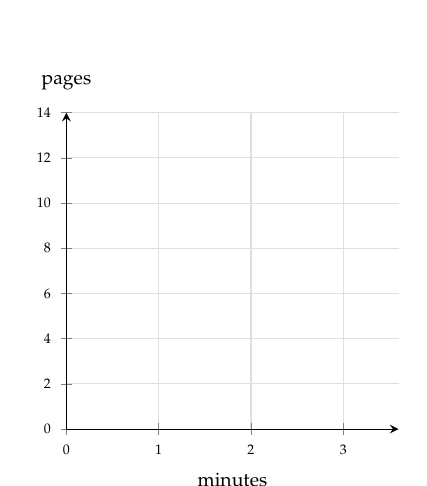
\begin{tikzpicture}
\begin{axis}[width=5.8cm,height=5.6cm,axis lines=left,xmin=0,xmax=3.6,ymin=0,ymax=14,xtick={0,...,3},ytick={0,2,...,14},
  grid=both,grid style={gray!25},xlabel={\scriptsize minutes},ylabel={\scriptsize pages},tick label style={font=\tiny},
  ylabel style={rotate=-90,at={(axis description cs:0,1.04)},anchor=south}]
\ifkey\addplot[FangBlue,thick,domain=0:3.3]{4*x};\addplot[only marks,mark=*,mark options={fill=FangBlue,draw=FangBlue}] coordinates{(0,0)(1,4)(2,8)(3,12)};\fi
\end{axis}
\end{tikzpicture}
\end{minipage}
\np[5.6cm]\item \begin{minipage}[t]{0.52\textwidth}\vspace{0pt}
Which graph shows a proportional relationship? For that one, find the constant of proportionality $k$.
\work[0.2cm]{Graph \textbf{B}: a straight line through the origin, through $(2,5)$, so $k=\tfrac52=2.5$. \ Graph A is a straight line but starts at $(0,2)$, so it is \textbf{not} proportional.}
\end{minipage}\hfill
\begin{minipage}[t]{0.44\textwidth}\vspace{0pt}\centering
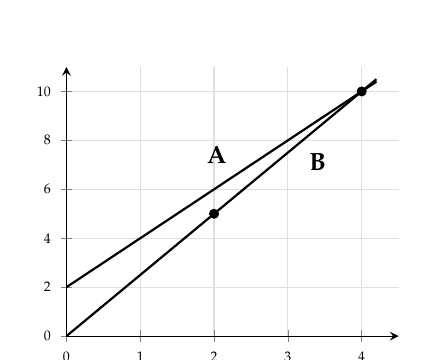
\begin{tikzpicture}
\begin{axis}[width=5.8cm,height=5cm,axis lines=left,xmin=0,xmax=4.5,ymin=0,ymax=11,xtick={0,...,4},ytick={0,2,...,10},
  grid=both,grid style={gray!25},tick label style={font=\tiny}]
\addplot[FangRed,thick,domain=0:4.2]{2*x+2} node[pos=0.55,above left,font=\small\bfseries]{A};
\addplot[FangBlue,thick,domain=0:4.2]{2.5*x} node[pos=0.75,below right,font=\small\bfseries]{B};
\addplot[only marks,mark=*,mark size=1.6pt,mark options={fill=FangBlue,draw=FangBlue}] coordinates{(2,5)(4,10)};
\end{axis}
\end{tikzpicture}
\end{minipage}
\np[3cm]\item \hard\ A proportional graph passes through $(6,\,15)$. Find $k$, write the equation, and find $y$ when $x=10$.
\work[1.6cm]{$k=\dfrac{15}{6}=2.5$. \ $y=2.5x$. \ When $x=10$: $y=25$. \ (Check: $(2,5)$ is also on the line, $5\div2=2.5$ \checkmark)}
\end{enumerate}

\needspace{5cm}{\large\bfseries\color{FangBlue}G.\ Challenge} \hard

\begin{enumerate}[resume,leftmargin=*,label=\textbf{\arabic*.},itemsep=6pt]
\np[3cm]\item Point $P(-3,\,a)$ is $7$ units from $Q(-3,\,2)$. Find \textbf{both} possible values of $a$.
\work[1.6cm]{Same $x$, so $|a-2|=7$: \ $a=2+7=9$ or $a=2-7=-5$. \ Points $(-3,9)$ and $(-3,-5)$.}
\np[3cm]\item The rectangle $(1,1)$, $(5,1)$, $(5,3)$, $(1,3)$ is reflected over the $y$-axis. List the new vertices. Did the area change?
\work[1.6cm]{$(-1,1)$, $(-5,1)$, $(-5,3)$, $(-1,3)$. The area stays $4\times2=8$ square units — a reflection flips the shape but does not change its size.}
\end{enumerate}

\ifkey\else
\vfill
\begin{simple}
\textbf{Before the test:} $x$ first, then $y$ \;·\; quadrants go counterclockwise from top right \;·\; across an axis, \textbf{add} distances \;·\; proportional = straight line \textbf{through the origin}, unit rate at $(1,k)$.
\end{simple}
\fi

\end{document}
"
% =====================================================================
\documentclass[12pt,letterpaper]{article}
\usepackage[margin=0.8in,top=0.85in,bottom=0.8in]{geometry}
\usepackage{mathpazo}
\usepackage[T1]{fontenc}
\usepackage{amsmath,amssymb}
\usepackage{xcolor}
\usepackage{enumitem}
\usepackage{multicol}
\usepackage{booktabs}
\usepackage{needspace}
\usepackage{fancyhdr}
\usepackage[most]{tcolorbox}
\usepackage{pgfplots}
\pgfplotsset{compat=1.17}
\usetikzlibrary{arrows.meta,calc}

\definecolor{FangBlue}{HTML}{000000}
\definecolor{FangTeal}{HTML}{000000}
\definecolor{FangGold}{HTML}{555555}
\definecolor{FangRed}{HTML}{000000}
\definecolor{FangGreen}{HTML}{000000}
\definecolor{FangPurple}{HTML}{000000}
\definecolor{Soft}{HTML}{FFFFFF}

\newif\ifkey
\ifdefined\iskey \keytrue \else \keyfalse \fi

\pagestyle{fancy}\fancyhf{}
\renewcommand{\headrulewidth}{0.4pt}
\fancyhead[L]{\small\color{FangBlue}\textbf{Prof. Fang Math} \,|\, Grade 7 \,·\, Graphing on the Coordinate Plane}
\fancyhead[R]{\small\ifkey\textcolor{FangRed}{\textbf{ANSWER KEY}}\else Name: \underline{\hspace{4.2cm}}\fi}
\fancyfoot[C]{\small\thepage}
\fancyfoot[R]{\scriptsize\color{gray}fangmath.com}
\setlength{\headheight}{14pt}
\setlength{\parindent}{0pt}
\setlength{\parskip}{4pt}

% ---------- boxes ----------
\newtcolorbox{idea}[1][]{colback=Soft,colframe=FangBlue,boxrule=0.8pt,arc=3pt,left=8pt,right=8pt,top=6pt,bottom=6pt,
  fonttitle=\bfseries,coltitle=white,colbacktitle=FangBlue,title={#1}}
\newtcolorbox{example}[1][]{colback=white,colframe=FangTeal,boxrule=0.6pt,arc=3pt,left=8pt,right=8pt,top=5pt,bottom=5pt,
  fonttitle=\bfseries,coltitle=FangTeal,colbacktitle=white,title={#1},attach boxed title to top left={xshift=8pt,yshift=-7pt},boxed title style={boxrule=0pt,colframe=white}, enhanced}
\newtcolorbox{warn}{colback=FangRed!5,colframe=FangRed,boxrule=0.6pt,arc=3pt,left=8pt,right=8pt,top=4pt,bottom=4pt,leftrule=3pt}
\newtcolorbox{simple}{colback=FangGold!10,colframe=FangGold,boxrule=0.6pt,arc=3pt,left=8pt,right=8pt,top=4pt,bottom=4pt,leftrule=3pt}
\newtcolorbox{sol}{colback=FangGreen!6,colframe=FangGreen,boxrule=0.5pt,arc=2pt,left=6pt,right=6pt,top=3pt,bottom=3pt,breakable}

\newcommand{\badge}[2]{\tcbox[on line,colback=#1,colframe=#1,coltext=white,boxrule=0pt,arc=6pt,left=4pt,right=4pt,top=1pt,bottom=1pt,fontupper=\scriptsize\bfseries]{#2}}
\newcommand{\easy}{\badge{FangGreen}{EASY}}
\newcommand{\medium}{\badge{FangTeal}{MEDIUM}}
\newcommand{\hard}{\badge{FangRed}{HARD}}
\newcommand{\work}[2][]{\ifkey\begin{sol}#2\end{sol}\else\vspace*{#1}\fi}
\newcommand{\np}[1][6cm]{\needspace{#1}}
\newcommand{\sect}[2]{\par\needspace{7cm}\medskip{\Large\bfseries\color{FangBlue}\tcbox[on line,colback=FangBlue,colframe=FangBlue,coltext=white,arc=2pt,boxrule=0pt,left=5pt,right=5pt,top=1pt,bottom=1pt]{#1}\ #2}\par\smallskip}

% ---------- right-triangle picture: \rt{scale}{a}{b}{labels...} ----------
% vertices: C = right angle at origin, A = (b,0) [the angle we look from], B = (0,a)
% ---------- coordinate grid: \cg[size]{xmin}{xmax}{ymin}{ymax}{plot commands} ----------
\newcommand{\cg}[6][5.4cm]{\begin{tikzpicture}\begin{axis}[width=#1,height=#1,axis lines=middle,
  xmin=#2-0.6,xmax=#3+0.6,ymin=#4-0.6,ymax=#5+0.6,xtick={#2,...,#3},ytick={#4,...,#5},
  grid=both,grid style={gray!28},xlabel={\scriptsize$x$},ylabel={\scriptsize$y$},
  tick label style={font=\tiny},axis line style={-{Stealth[length=4pt]},thick},clip=false,
  xticklabel style={fill=white,inner sep=1pt},yticklabel style={fill=white,inner sep=1pt}]#6\end{axis}\end{tikzpicture}}
\newcommand{\pt}[4][FangBlue]{\fill[#1](axis cs:#2,#3) circle(2.3pt) node[above right,font=\scriptsize\bfseries,text=#1,inner sep=1.5pt]{#4};}
\newcommand{\blank}{\underline{\hspace{1.6cm}}}

\begin{document}

% ======================= TITLE =======================
\begin{center}
{\color{FangBlue}\Huge\bfseries Graphing on the Coordinate Plane}\\[3pt]
{\large Test review: points, quadrants, reflections, distance, shapes and proportional graphs}
\ifkey\\[3pt]{\color{FangRed}\large\bfseries Answer Key}\fi
\end{center}
\vspace{-2pt}

% ======================= PART 1 =======================
\sect{1}{The coordinate plane}

\begin{minipage}[c]{0.46\textwidth}\centering
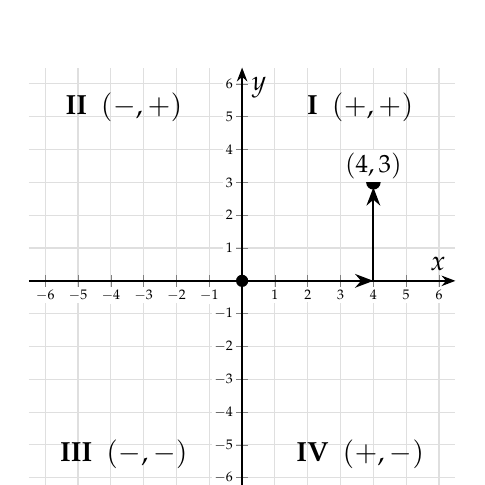
\begin{tikzpicture}
\begin{axis}[width=7cm,height=7cm,axis lines=middle,xmin=-6.5,xmax=6.5,ymin=-6.5,ymax=6.5,
  xtick={-6,...,6},ytick={-6,...,6},grid=both,grid style={gray!25},xlabel={$x$},ylabel={$y$},
  tick label style={font=\tiny},axis line style={-{Stealth[length=5pt]},thick},
  xticklabel style={fill=white,inner sep=1pt},yticklabel style={fill=white,inner sep=1pt}]
\node[FangTeal,font=\bfseries] at (axis cs:3.6,5.3) {I \ $(+,+)$};
\node[FangTeal,font=\bfseries] at (axis cs:-3.6,5.3) {II \ $(-,+)$};
\node[FangTeal,font=\bfseries] at (axis cs:-3.6,-5.3) {III \ $(-,-)$};
\node[FangTeal,font=\bfseries] at (axis cs:3.6,-5.3) {IV \ $(+,-)$};
\draw[FangRed,thick,-{Stealth}] (axis cs:0,0) -- (axis cs:4,0);
\draw[FangRed,thick,-{Stealth}] (axis cs:4,0) -- (axis cs:4,2.85);
\fill[FangRed](axis cs:4,3) circle(2.6pt) node[above,font=\small\bfseries,fill=white,inner sep=1pt]{$(4,3)$};
\fill(axis cs:0,0) circle(2.2pt);
\end{axis}
\end{tikzpicture}
\end{minipage}\hfill
\begin{minipage}[c]{0.52\textwidth}
\begin{itemize}[leftmargin=*,itemsep=3pt]
\item The \textbf{$x$-axis} goes left–right; the \textbf{$y$-axis} goes up–down. They cross at the \textbf{origin} $(0,0)$.
\item An \textbf{ordered pair} $(x,\,y)$: \textbf{first} walk left/right ($x$), \textbf{then} up/down ($y$). \\
\emph{“Walk to the elevator, then ride it.”}
\item The axes cut the plane into four \textbf{quadrants}, numbered I–IV \textbf{counterclockwise}, starting at the top right.
\item A point \textbf{on an axis} (like $(0,5)$ or $(-2,0)$) is in \textbf{no} quadrant.
\end{itemize}
\end{minipage}

\begin{warn}
\textbf{Watch out:} $(4,3)$ and $(3,4)$ are \textbf{different} points. Order matters: $x$ always comes first.
\end{warn}

% ======================= PART 2 =======================
\sect{2}{Reflections — flip over an axis}

\begin{minipage}[c]{0.46\textwidth}\centering
\cg[6.4cm]{-5}{5}{-5}{5}{
\pt[FangBlue]{3}{2}{$A(3,2)$}
\fill[FangRed](axis cs:3,-2) circle(2.3pt) node[below right,font=\scriptsize\bfseries,text=FangRed]{$(3,-2)$};
\fill[FangGreen](axis cs:-3,2) circle(2.3pt) node[above left,font=\scriptsize\bfseries,text=FangGreen]{$(-3,2)$};
\draw[FangRed,dashed](axis cs:3,2)--(axis cs:3,-2);
\draw[FangGreen,dashed](axis cs:3,2)--(axis cs:-3,2);}
\end{minipage}\hfill
\begin{minipage}[c]{0.52\textwidth}
\renewcommand{\arraystretch}{1.35}
\begin{tabular}{@{}lll@{}}
\toprule
\textbf{Reflect over\ldots} & \textbf{Rule} & \textbf{Example}\\ \midrule
\textcolor{FangRed}{the $x$-axis} & $(x,y)\to(x,\,-y)$ & $(3,2)\to(3,-2)$\\
\textcolor{FangGreen}{the $y$-axis} & $(x,y)\to(-x,\,y)$ & $(3,2)\to(-3,2)$\\
\bottomrule
\end{tabular}\par\medskip
\textbf{Memory trick:} over the \textbf{$x$-axis}, the \textbf{$x$ stays}; only $y$ changes sign. Over the \textbf{$y$-axis}, the \textbf{$y$ stays}.
\end{minipage}

% ======================= PART 3 =======================
\sect{3}{Distance between two points on a line}

\begin{idea}[Same $x$ or same $y$? Count — or use absolute value]
\textbf{Same quadrant / same side:} subtract. \quad $(2,5)$ to $(2,1)$: \ $5-1=4$ units.\par
\textbf{Opposite sides of an axis:} \textbf{add} the absolute values. \quad $(-3,4)$ to $(5,4)$: \ $|-3|+|5|=3+5=8$ units.\par
One rule for both: \textbf{distance} $=|\,\text{difference}\,|$. \quad $|5-(-3)|=|8|=8$. \ \ Distance is never negative.
\end{idea}

\begin{simple}
\textbf{Simple case first:} from $(-1,0)$ to $(1,0)$ — count the squares: $2$. And $|-1|+|1|=2$ \checkmark. That's why you \textbf{add} across the axis.
\end{simple}

% ======================= PART 4 =======================
\sect{4}{Shapes on the coordinate plane}

\begin{example}[Example \;·\; rectangle $ABCD$ with $A(-3,2)$, $B(4,2)$, $C(4,-1)$, $D(-3,-1)$]
\begin{minipage}[c]{0.4\textwidth}\centering
\cg[5.6cm]{-4}{5}{-2}{3}{
\draw[FangBlue,thick,fill=FangBlue!8](axis cs:-3,2)--(axis cs:4,2)--(axis cs:4,-1)--(axis cs:-3,-1)--cycle;
\pt{-3}{2}{A}\pt{4}{2}{B}\pt{4}{-1}{C}\pt{-3}{-1}{D}}
\end{minipage}\hfill
\begin{minipage}[c]{0.56\textwidth}
Length $AB$: same $y$, so $|4-(-3)|=7$. \\
Width $BC$: same $x$, so $|2-(-1)|=3$. \\[3pt]
\textbf{Perimeter} $=7+3+7+3=20$ units. \\
\textbf{Area} $=7\times3=21$ square units.
\end{minipage}
\end{example}

% ======================= PART 5 =======================
\sect{5}{Graphing a proportional relationship}

\begin{example}[Example \;·\; Tickets cost \$3 each]
\begin{minipage}[c]{0.42\textwidth}\centering
\begin{tabular}{c|ccccc}
tickets $x$ & 0 & 1 & 2 & 3 & 4\\ \hline
cost $y$ (\$) & 0 & 3 & 6 & 9 & 12
\end{tabular}\\[6pt]
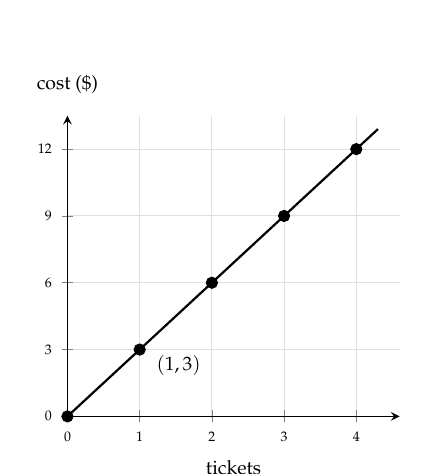
\begin{tikzpicture}
\begin{axis}[width=5.8cm,height=5.4cm,axis lines=left,xmin=0,xmax=4.6,ymin=0,ymax=13.5,xtick={0,...,4},ytick={0,3,...,12},
  grid=both,grid style={gray!25},xlabel={\scriptsize tickets},ylabel={\scriptsize cost (\$)},tick label style={font=\tiny},
  ylabel style={rotate=-90,at={(axis description cs:0,1.04)},anchor=south}]
\addplot[FangBlue,thick,domain=0:4.3]{3*x};
\addplot[only marks,mark=*,mark options={fill=FangBlue,draw=FangBlue}] coordinates{(0,0)(1,3)(2,6)(3,9)(4,12)};
\node[FangRed,font=\scriptsize\bfseries,anchor=west] at (axis cs:1.1,2.3) {$(1,3)$};
\end{axis}
\end{tikzpicture}
\end{minipage}\hfill
\begin{minipage}[c]{0.55\textwidth}
\textbf{How to tell it's proportional from a graph:}
\begin{enumerate}[leftmargin=*,itemsep=2pt]
\item the points are on a \textbf{straight line}, and
\item the line goes \textbf{through the origin} $(0,0)$.
\end{enumerate}
The \textbf{constant of proportionality} (unit rate) is $k=\dfrac{y}{x}=\dfrac{3}{1}=3$. Equation: $y=3x$.\par
\textbf{Look for the point $(1,\,k)$}: here $(1,3)$ means \emph{1 ticket costs \$3}.\par
A point like $(4,12)$ means \emph{4 tickets cost \$12}.
\end{minipage}
\end{example}

\begin{warn}
\textbf{Not proportional:} a straight line that \textbf{doesn't} pass through $(0,0)$ — for example a \$5 entry fee plus \$3 per ride: $y=3x+5$ starts at $(0,5)$.
\end{warn}

% ======================= PRACTICE =======================
\sect{6}{Practice}
\ifkey\else\textit{Show your work. Label every point you plot.}\fi

\needspace{8cm}{\large\bfseries\color{FangBlue}A.\ Read and plot points} \easy

\begin{minipage}[t]{0.42\textwidth}\vspace{0pt}\centering
\cg[6.2cm]{-6}{6}{-6}{6}{
\pt{2}{5}{A}\pt{-4}{3}{B}\pt{-3}{-2}{C}\pt{5}{-4}{D}\pt{0}{-5}{E}\pt{-6}{0}{F}
\ifkey
\pt[FangRed]{3}{1}{P}\pt[FangRed]{-5}{-4}{Q}\pt[FangRed]{0}{4}{R}\pt[FangRed]{4}{-2}{S}
\fi}
\end{minipage}\hfill
\begin{minipage}[t]{0.55\textwidth}\vspace{2pt}
\begin{enumerate}[leftmargin=*,label=\textbf{\arabic*.},itemsep=5pt]
\item Write the coordinates of each point.\\[3pt]
$A$ \ifkey\textcolor{FangGreen}{$(2,5)$}\else\blank\fi \quad $B$ \ifkey\textcolor{FangGreen}{$(-4,3)$}\else\blank\fi \\[3pt]
$C$ \ifkey\textcolor{FangGreen}{$(-3,-2)$}\else\blank\fi \quad $D$ \ifkey\textcolor{FangGreen}{$(5,-4)$}\else\blank\fi \\[3pt]
$E$ \ifkey\textcolor{FangGreen}{$(0,-5)$}\else\blank\fi \quad $F$ \ifkey\textcolor{FangGreen}{$(-6,0)$}\else\blank\fi
\item Which quadrant is each of $A$, $B$, $C$, $D$ in? Which points are on an axis?
\work[1.2cm]{$A$: I, \ $B$: II, \ $C$: III, \ $D$: IV. \ $E$ and $F$ are on an axis (no quadrant).}
\item Plot and label on the same grid: \\ $P(3,1)$, \ $Q(-5,-4)$, \ $R(0,4)$, \ $S(4,-2)$.
\work[0.4cm]{Points $P$, $Q$, $R$, $S$ are plotted on the grid.}
\end{enumerate}
\end{minipage}

\needspace{5cm}{\large\bfseries\color{FangBlue}B.\ Signs and quadrants} \easy\ \medium

\begin{enumerate}[start=4,leftmargin=*,label=\textbf{\arabic*.},itemsep=5pt]
\np[2cm]\item Name the quadrant: \quad (a) $(-7,\,2)$ \quad (b) $(6,\,-1)$ \quad (c) $(-0.5,\,-8)$ \quad (d) $(3\tfrac12,\,4)$
\work[1cm]{(a) II \quad (b) IV \quad (c) III \quad (d) I}
\np[2cm]\item A point has a negative $x$-coordinate and a positive $y$-coordinate. Which quadrant is it in?
\work[1cm]{Quadrant II \ $(-,+)$.}
\np[2cm]\item True or false: the point $(0,-3)$ is in Quadrant IV. Explain.
\work[1.2cm]{False. Its $x$-coordinate is $0$, so it lies \textbf{on the $y$-axis} — in no quadrant.}
\end{enumerate}

\needspace{5cm}{\large\bfseries\color{FangBlue}C.\ Reflections} \medium

\begin{enumerate}[resume,leftmargin=*,label=\textbf{\arabic*.},itemsep=5pt]
\np[2cm]\item Reflect $(5,-2)$ over the $x$-axis. \quad Then reflect $(5,-2)$ over the $y$-axis.
\work[1cm]{Over the $x$-axis: $(5,2)$. \quad Over the $y$-axis: $(-5,-2)$.}
\np[2cm]\item $(-4,\,6)$ is reflected over the $y$-axis, and then the new point is reflected over the $x$-axis. Where does it end up? Which quadrant?
\work[1.4cm]{$(-4,6)\to(4,6)\to(4,-6)$. \ Quadrant IV. (Two flips change both signs.)}
\np[2cm]\item Point $M$ is $(a,\,b)$ and point $N$ is $(a,\,-b)$. Over which axis is $N$ the reflection of $M$?
\work[1cm]{The $x$-axis (the $x$-coordinate stayed the same).}
\end{enumerate}

\needspace{5cm}{\large\bfseries\color{FangBlue}D.\ Distance} \medium

\begin{enumerate}[resume,leftmargin=*,label=\textbf{\arabic*.},itemsep=5pt]
\np[2cm]\item Find the distance between $(3,\,7)$ and $(3,\,-2)$.
\work[1.2cm]{Same $x$. Opposite sides of the $x$-axis: $7+2=9$ units. \ (Or $|7-(-2)|=9$.)}
\np[2cm]\item Find the distance between $(-6,\,-1)$ and $(-2,\,-1)$.
\work[1.2cm]{Same $y$. Same side: $|-2-(-6)|=|4|=4$ units.}
\np[2cm]\item Point $A$ is at $(-5,\,4)$. Point $B$ is $9$ units to the right of $A$. Find $B$. Which quadrant is $B$ in?
\work[1.2cm]{$B=(-5+9,\,4)=(4,4)$, \ Quadrant I.}
\np[2.4cm]\item A diver is at $-12$ m and a seagull is at $+15$ m, straight above the diver. How far apart are they?
\work[1.2cm]{$|-12|+|15|=12+15=27$ m (opposite sides of sea level, so add).}
\end{enumerate}

\needspace{7cm}{\large\bfseries\color{FangBlue}E.\ Shapes} \medium\ \hard

\begin{enumerate}[resume,leftmargin=*,label=\textbf{\arabic*.},itemsep=6pt]
\np[5cm]\item \begin{minipage}[t]{0.5\textwidth}\vspace{0pt}
Plot $J(-4,3)$, $K(2,3)$, $L(2,-2)$ and $M(-4,-2)$ and connect them in order. \\
(a) What shape is $JKLM$? \\ (b) Find its perimeter. \\ (c) Find its area.
\work[0.2cm]{(a) A rectangle. \ (b) $JK=|2-(-4)|=6$, $KL=|3-(-2)|=5$. Perimeter $=2(6+5)=22$ units. \ (c) Area $=6\times5=30$ square units.}
\end{minipage}\hfill
\begin{minipage}[t]{0.42\textwidth}\vspace{0pt}\centering
\cg[5.6cm]{-5}{5}{-5}{5}{\ifkey\draw[FangBlue,thick,fill=FangBlue!8](axis cs:-4,3)--(axis cs:2,3)--(axis cs:2,-2)--(axis cs:-4,-2)--cycle;\pt{-4}{3}{J}\pt{2}{3}{K}\pt{2}{-2}{L}\pt{-4}{-2}{M}\fi}
\end{minipage}
\np[2.6cm]\item Three corners of a square are $(-1,4)$, $(3,4)$ and $(3,0)$. Find the fourth corner and the area of the square.
\work[1.4cm]{The fourth corner is $(-1,0)$. Side $=|3-(-1)|=4$, so area $=4\times4=16$ square units.}
\np[3cm]\item \hard\ A triangle has vertices $(-2,-3)$, $(4,-3)$ and $(1,5)$. Find its area.
\work[1.6cm]{Base on $y=-3$: $|4-(-2)|=6$. Height: from $y=-3$ up to $y=5$ is $|5-(-3)|=8$. \ Area $=\tfrac12\cdot6\cdot8=24$ square units.}
\end{enumerate}

\needspace{8cm}{\large\bfseries\color{FangBlue}F.\ Proportional relationships} \medium\ \hard

\begin{enumerate}[resume,leftmargin=*,label=\textbf{\arabic*.},itemsep=6pt]
\np[6.5cm]\item \begin{minipage}[t]{0.52\textwidth}\vspace{0pt}
A printer prints $4$ pages per minute. \\[2pt]
\begin{tabular}{c|cccc}minutes $x$ & 0 & 1 & 2 & 3\\ \hline pages $y$ & \ifkey 0\else\fi & \ifkey 4\else\fi & \ifkey 8\else\fi & \ifkey 12\else\fi\end{tabular}\\[4pt]
(a) Complete the table and graph it. \\
(b) Is the relationship proportional? How can you tell from the graph? \\
(c) Write an equation. \quad (d) What does the point $(1,4)$ mean?
\work[0.2cm]{(b) Yes — the points make a straight line through $(0,0)$. \ (c) $y=4x$. \ (d) In $1$ minute the printer prints $4$ pages (the unit rate).}
\end{minipage}\hfill
\begin{minipage}[t]{0.44\textwidth}\vspace{0pt}\centering
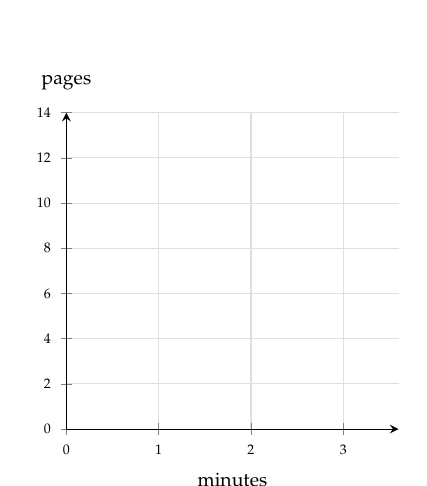
\begin{tikzpicture}
\begin{axis}[width=5.8cm,height=5.6cm,axis lines=left,xmin=0,xmax=3.6,ymin=0,ymax=14,xtick={0,...,3},ytick={0,2,...,14},
  grid=both,grid style={gray!25},xlabel={\scriptsize minutes},ylabel={\scriptsize pages},tick label style={font=\tiny},
  ylabel style={rotate=-90,at={(axis description cs:0,1.04)},anchor=south}]
\ifkey\addplot[FangBlue,thick,domain=0:3.3]{4*x};\addplot[only marks,mark=*,mark options={fill=FangBlue,draw=FangBlue}] coordinates{(0,0)(1,4)(2,8)(3,12)};\fi
\end{axis}
\end{tikzpicture}
\end{minipage}
\np[5.6cm]\item \begin{minipage}[t]{0.52\textwidth}\vspace{0pt}
Which graph shows a proportional relationship? For that one, find the constant of proportionality $k$.
\work[0.2cm]{Graph \textbf{B}: a straight line through the origin, through $(2,5)$, so $k=\tfrac52=2.5$. \ Graph A is a straight line but starts at $(0,2)$, so it is \textbf{not} proportional.}
\end{minipage}\hfill
\begin{minipage}[t]{0.44\textwidth}\vspace{0pt}\centering
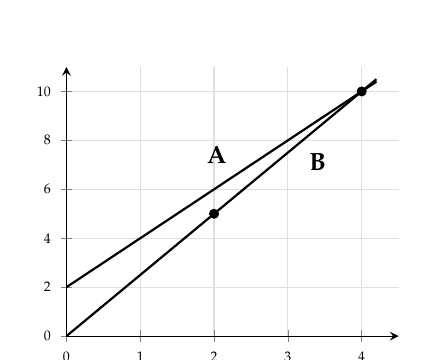
\begin{tikzpicture}
\begin{axis}[width=5.8cm,height=5cm,axis lines=left,xmin=0,xmax=4.5,ymin=0,ymax=11,xtick={0,...,4},ytick={0,2,...,10},
  grid=both,grid style={gray!25},tick label style={font=\tiny}]
\addplot[FangRed,thick,domain=0:4.2]{2*x+2} node[pos=0.55,above left,font=\small\bfseries]{A};
\addplot[FangBlue,thick,domain=0:4.2]{2.5*x} node[pos=0.75,below right,font=\small\bfseries]{B};
\addplot[only marks,mark=*,mark size=1.6pt,mark options={fill=FangBlue,draw=FangBlue}] coordinates{(2,5)(4,10)};
\end{axis}
\end{tikzpicture}
\end{minipage}
\np[3cm]\item \hard\ A proportional graph passes through $(6,\,15)$. Find $k$, write the equation, and find $y$ when $x=10$.
\work[1.6cm]{$k=\dfrac{15}{6}=2.5$. \ $y=2.5x$. \ When $x=10$: $y=25$. \ (Check: $(2,5)$ is also on the line, $5\div2=2.5$ \checkmark)}
\end{enumerate}

\needspace{5cm}{\large\bfseries\color{FangBlue}G.\ Challenge} \hard

\begin{enumerate}[resume,leftmargin=*,label=\textbf{\arabic*.},itemsep=6pt]
\np[3cm]\item Point $P(-3,\,a)$ is $7$ units from $Q(-3,\,2)$. Find \textbf{both} possible values of $a$.
\work[1.6cm]{Same $x$, so $|a-2|=7$: \ $a=2+7=9$ or $a=2-7=-5$. \ Points $(-3,9)$ and $(-3,-5)$.}
\np[3cm]\item The rectangle $(1,1)$, $(5,1)$, $(5,3)$, $(1,3)$ is reflected over the $y$-axis. List the new vertices. Did the area change?
\work[1.6cm]{$(-1,1)$, $(-5,1)$, $(-5,3)$, $(-1,3)$. The area stays $4\times2=8$ square units — a reflection flips the shape but does not change its size.}
\end{enumerate}

\ifkey\else
\vfill
\begin{simple}
\textbf{Before the test:} $x$ first, then $y$ \;·\; quadrants go counterclockwise from top right \;·\; across an axis, \textbf{add} distances \;·\; proportional = straight line \textbf{through the origin}, unit rate at $(1,k)$.
\end{simple}
\fi

\end{document}
